\documentclass[table, 10pt]{beamer}%
%\documentclass[table, 10 pt, handout]{beamer}%

\usepackage[french]{babel}
\usepackage{tikz}
\usepackage[latin1]{inputenc}
\usepackage{times}
\usepackage[T1]{fontenc}

\usepackage{graphicx,graphics}

\usepackage{amsmath,amsfonts}

\usepackage{multirow}

%\usepackage[table]{xcolor}

%\usepackage{beamerthemeliris}

\usepackage{beamerthemesplit}
\usetheme{JuanLesPins}%Copenhagen%Dresden%Malmoe
\usecolortheme{orchid}%beetle,seagull,crane,dove,orchid
\useinnertheme[shadow=true]{rounded}%rounded
\useoutertheme{miniframes}
\usefonttheme{professionalfonts}

\definecolor{darkgreen}{RGB}{0,180,0} 

\setbeamertemplate{navigation symbols}{}


%% Trop long 15 minutes


\title[S21 - Comprendre les r�seaux -- CM3 - IPv4\hspace{1cm}\insertframenumber{} / \inserttotalframenumber]
{S21 -- Comprendre les r�seaux }
\subtitle{CM3 -- Plan d'adressage et Services r�seaux}
\author[Julien Gossa]
{Julien Gossa}
\institute
{
	{\bf IUT Robert Schuman -- D�partement Informatique}\\
	{\url{julien.gossa@unistra.fr}}
}

\date{2010}
\beamertemplatetransparentcovereddynamicmedium 

\begin{document}


\begin{frame}
 	\titlepage
\end{frame}


%% ----------------------------------------------------------------------
%\begin{frame}
%
%	\begin{block}<+->{Intervenants}
%		\begin{itemize}
%		\item Julien Gossa \hfill \url{julien.gossa@unistra.fr}
%		\item Aur�lie Bertaux \hfill \url{aurelie.bertaux@unistra.fr}
%		\end{itemize}
%	\end{block}
%
%	\begin{block}<+-> {Planning}
%		\begin{itemize}
%		\item Introduction/Pr�sentation, manipulation et configuration 
%			\begin{itemize}
%			\item 1 TD : Protocole Ethernet				
%			\item 2 TP : Manipulation des commandes UNIX dans un script shell
%			\end{itemize}
%		\vspace{0.2cm}	
%		\item Architectures mat�rielles, conception et simulation
%			\begin{itemize}
%			\item 1 TD : Manipulation des adresses IPv4			
%			\item 1 TD : Plan d'adressage
%			\item 1 TD : Architecture PME
%			\item 2 TP : Impl�mentation au sein d'un simulateur
%			\end{itemize}		
%		\vspace{0.2cm}
%		\item Architectures logicielles, programmation client/serveur
%			\begin{itemize}
%			\item 2 TD : Initiation Perl et conception
%			\item 2 TP : Programmation client/serveur
%			\end{itemize}
%		\end{itemize}
%	\end{block}
%	
%\end{frame}
%% ----------------------------------------------------------------------

\AtBeginSection[]
{
   \begin{frame}
       \frametitle{Sans transition\ldots}
       \small
       \tableofcontents[hideothersubsections]
   \end{frame}
}	

%\def\resdir{1intro}

% ----------------------------------------------------------------------
\section{Introduction}
% ----------------------------------------------------------------------

% ----------------------------------------------------------------------
\subsection{Historique}
% ----------------------------------------------------------------------
\begin{frame}{Historique}
	
	\begin{itemize}
		\item<+-> 1968 : Arpanet (Advanced Research Projects Agency), DOD am�ricain, mel entre centres de recherche, protocole X25
		\item<+-> 1972 : protocole TCP/IP, r�sister � une attaque nucl�aire
		\item<+-> 1979 : mise en domaine public, r�cup�ration par les universit� (Duke University, Caroline du Nord), USENET (news)
		\item<+-> 1982 : acc�s gratuit au r�seau
		\item<+-> 1983 : arriv�e en Europe, CNAM en France, r�seau de r�seaux
		\item<+-> 1984 : ARPANET devient MILNET + INTERNET par la NFS
		\item<+-> 1986 : connexion aux lignes publiques
		\item<+-> 1991 : Apparition des FAI
		\item<+-> 1993 : WWW, 1ier navigateur au CERN, HTML/hyperliens
		\item<+-> 1995 : 2 millions d'ordinateurs, 30 millions d'utilisateurs
		\item<+-> 2008 : 15,5 millions de foyers haut-d�bit en France, +1milliard d'internautes dans le monde
	\end{itemize}

\end{frame}


% ----------------------------------------------------------------------
\begin{frame}{Nombre de sites Web}
	
	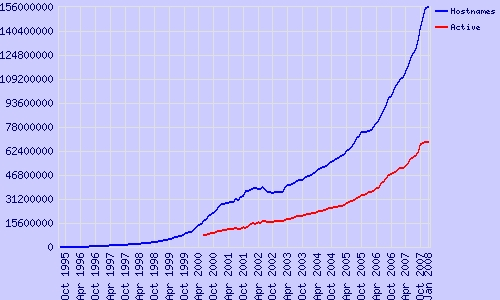
\includegraphics[width=\textwidth]{\resdir/sitecounthistory}
		
\end{frame}




% ----------------------------------------------------------------------
\subsection{Visualisation}
% ----------------------------------------------------------------------
\begin{frame}{\'Epine dorsale d'Internet}
	\centering
	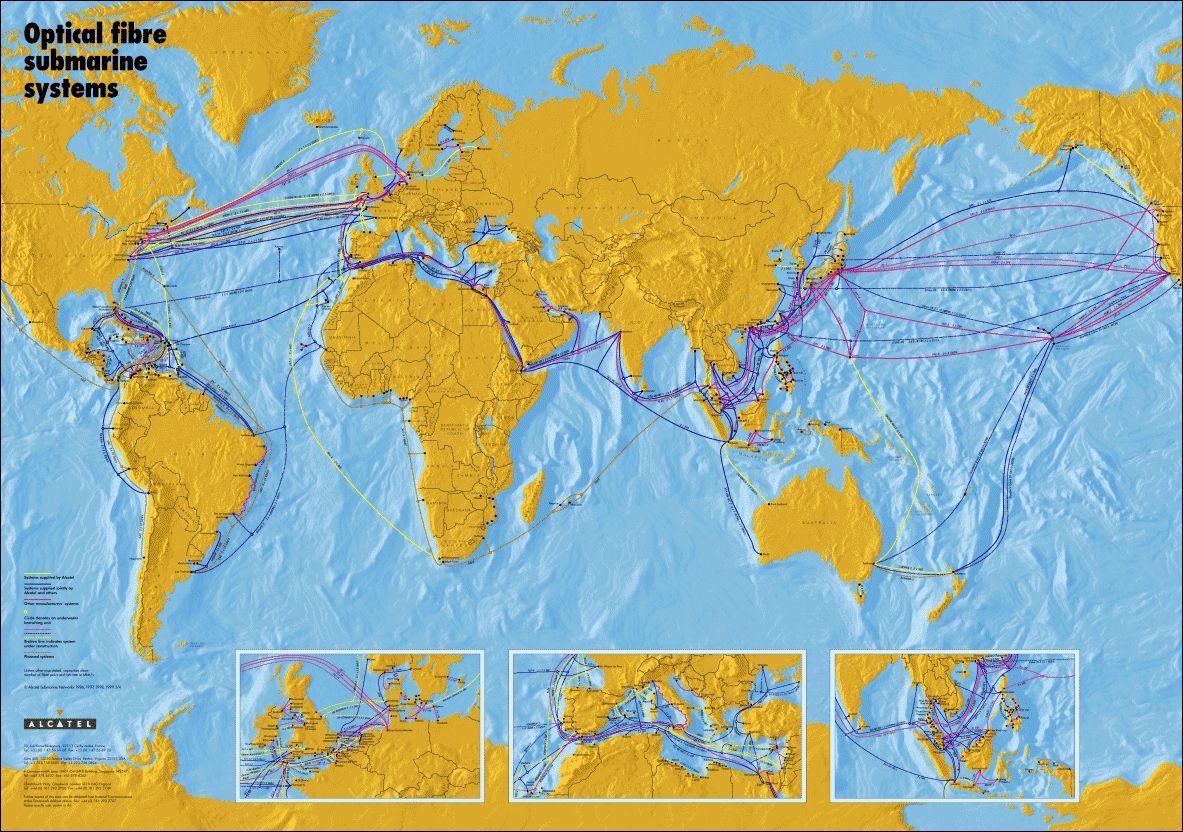
\includegraphics[width=\textwidth]{\resdir/carte-internet-backbone}
\end{frame}

\begin{frame}{Repr�sentation d'Internet}
	\centering
	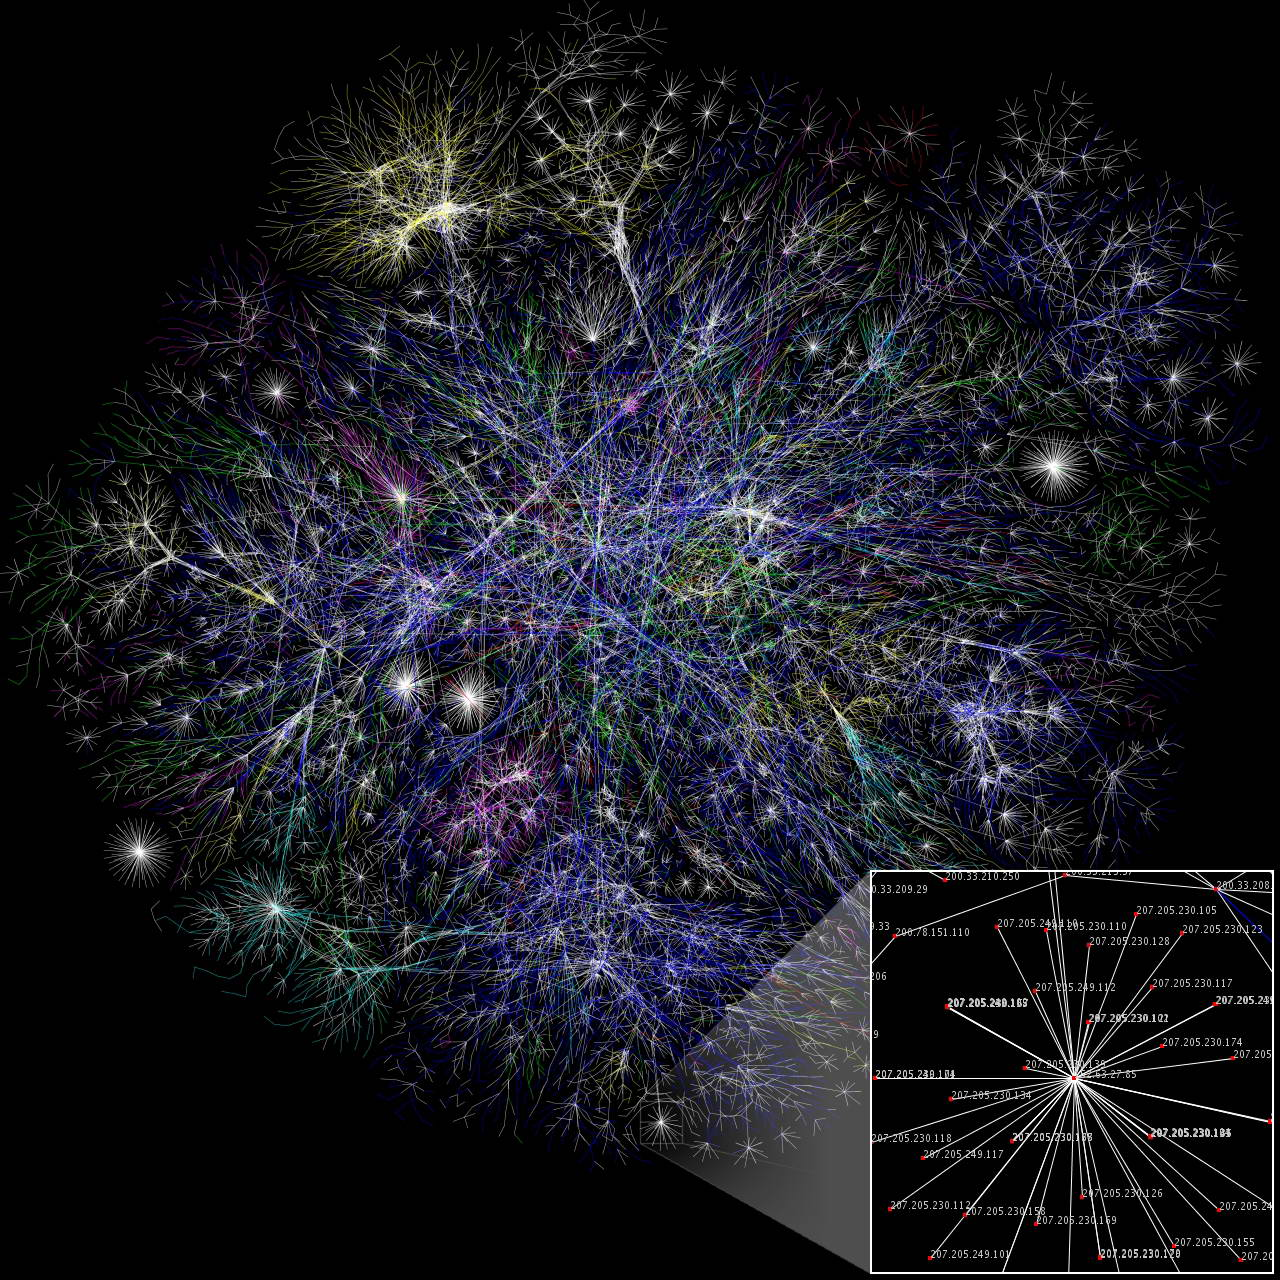
\includegraphics[height=0.8\textheight]{\resdir/carte-internet}
		
\end{frame}


% ----------------------------------------------------------------------
\begin{frame}
	
	\begin{block}<+-> {Caract�ristiques d'Internet}
		\begin{itemize}
		\item D�centralis� et dynamique : pas de point n�vralgique
		\item Construit par le bas : pas de planification globale
		\item Ensemble de domaines autonomes interconnect�s
		\item H�t�rog�ne : �quipement, utilisateur, utilisation\ldots
		\end{itemize}
	\end{block}
	
\end{frame}



% ----------------------------------------------------------------------
\subsection{APS}
% ----------------------------------------------------------------------
\begin{frame}
	\begin{block}<+-> {APS}
		\begin{itemize}
		\item Architecture : Infrastructure et mat�riel
		\item Protocole : langage de communication
		\item Service : applications
		\end{itemize}
		Doivent �tre norm�s (RFC : Request For comment)	
	\end{block}
\end{frame}

% ----------------------------------------------------------------------
\begin{frame}
	
	\begin{block}<+-> {Architecture Mat�rielle}
	
		\begin{itemize}
		
		\item Mat�riel d'extr�mit�
			\begin{itemize} 
			\item poste client, serveur\ldots
			\item utilisent le r�seau pour communiquer
			\end{itemize}
			
		\item Mat�riel internes 
			\begin{itemize} 
			\item routeur, DNS\ldots
			\item responsable de l'acheminement
			\end{itemize}	
			
		\item C�bles
			\begin{itemize} 
			\item responsable du transport entre deux points
			\end{itemize}
			
		\end{itemize}
		
	\end{block}
		
\end{frame}



% ----------------------------------------------------------------------
\begin{frame}
	
	\begin{block}<+-> {Protocoles}
		\begin{itemize}
		
		\item ensemble de r�gles et de conventions 
			\begin{itemize} 
			\item r�aliser les �changes d'informations
			\item = langage
			\item propri�taire ou ouvert
			\end{itemize}
			
		\item acteurs
			\begin{itemize} 
			\item constructeurs
			\item op�rateurs de t�l�communication
			\item utilisateurs, communaut�
			\end{itemize}	

		\item exemples 
			\begin{itemize} 
			\item TCP/UDP
			\item Kad
			\item IRC, MSN, Jabber
			\end{itemize}
		
		\end{itemize}
		
	\end{block}
\end{frame}


% ----------------------------------------------------------------------
\begin{frame}
	
	\begin{block}<+-> {Services}
		\begin{itemize}
		
		\item Applications
			\begin{itemize} 
			\item en mode client/serveur ou pair � pair
			\item distantes et � la disposition des utilisateurs
			\end{itemize}
			
		\item Exemples
			\begin{itemize} 
			\item Connexion distante
			\item Transfert de fichiers
			\item WWW, mel
			\item Annuaire
			\item Impression
			\item \ldots
			\end{itemize}	
		\end{itemize}
		
	\end{block}
\end{frame}


% ----------------------------------------------------------------------
\begin{frame}
	\begin{columns}
	
	\column{0.5\textwidth}
		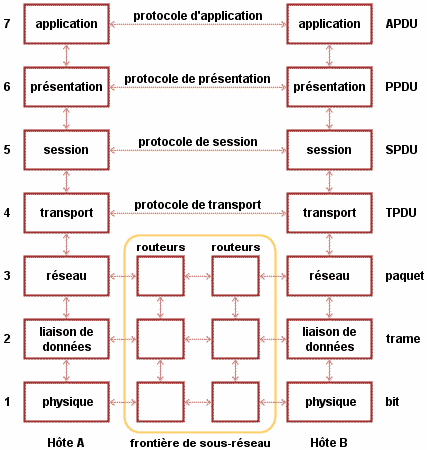
\includegraphics[height=0.8\textheight]{\resdir/osi}
	
	\column{0.5\textwidth}
		\begin{block}<+-> {Mod�le OSI}
			\begin{itemize}
				\item S�paration en couches
				\item Chacune rend un service � celle juste au dessus
				\item Les donn�es doivent traverser toutes les couches
				\item Avantages :
				\begin{itemize}
					\item R�duit la complexit�
					\item Uniformise les interfaces
					\item Assure l'interop�rabilit�
					\item Facilite la conception modulaire
					\item Acc�l�re l'�volution
				\end{itemize}
			\end{itemize}
		\end{block}
		
	\end{columns}


\end{frame}

%
%\def\resdir{2materiel}
\def\imgheight{0.4\textheight}

% ----------------------------------------------------------------------
\section{Architecture Mat�rielle}
% ----------------------------------------------------------------------


% ----------------------------------------------------------------------
\subsection{C�bles}
% ----------------------------------------------------------------------
\begin{frame}

\centering
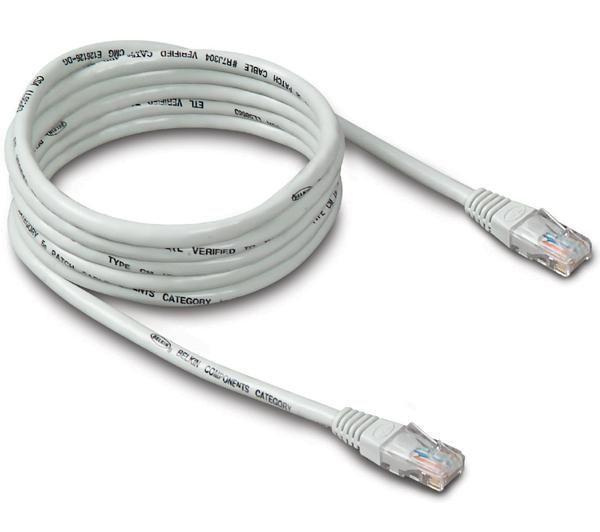
\includegraphics[height=0.4\textheight]{\resdir/cablerj45.jpg}\hfill
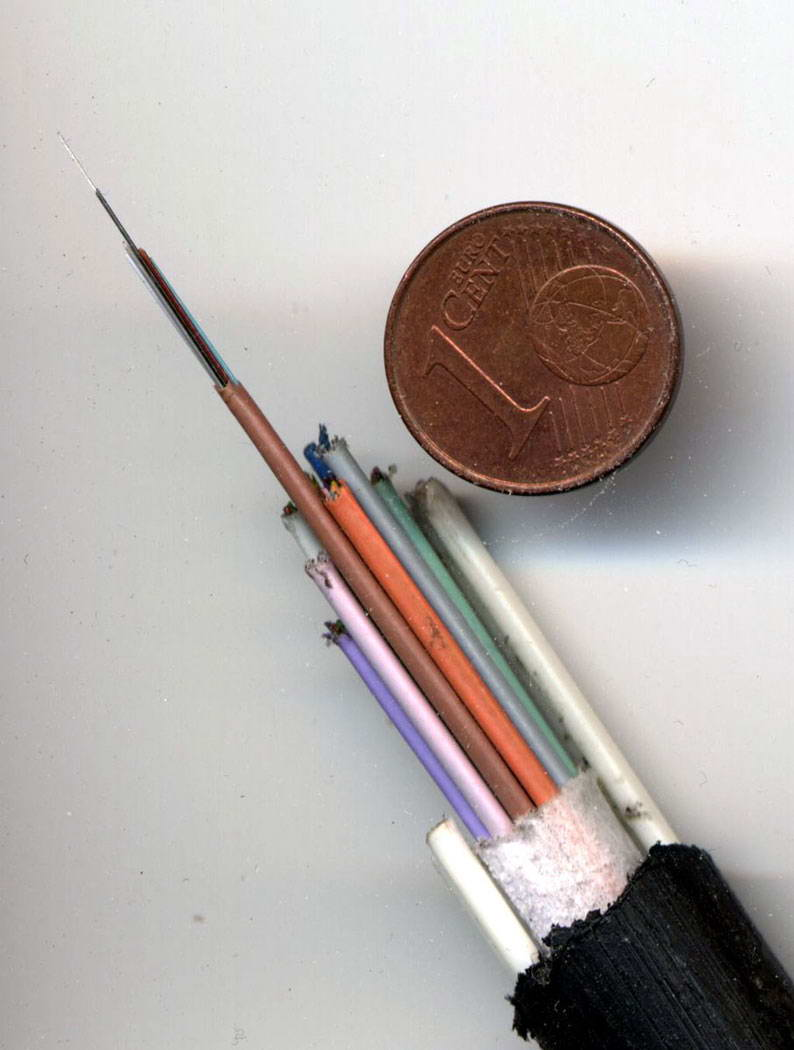
\includegraphics[height=0.4\textheight]{\resdir/cablefo.jpg}\hfill
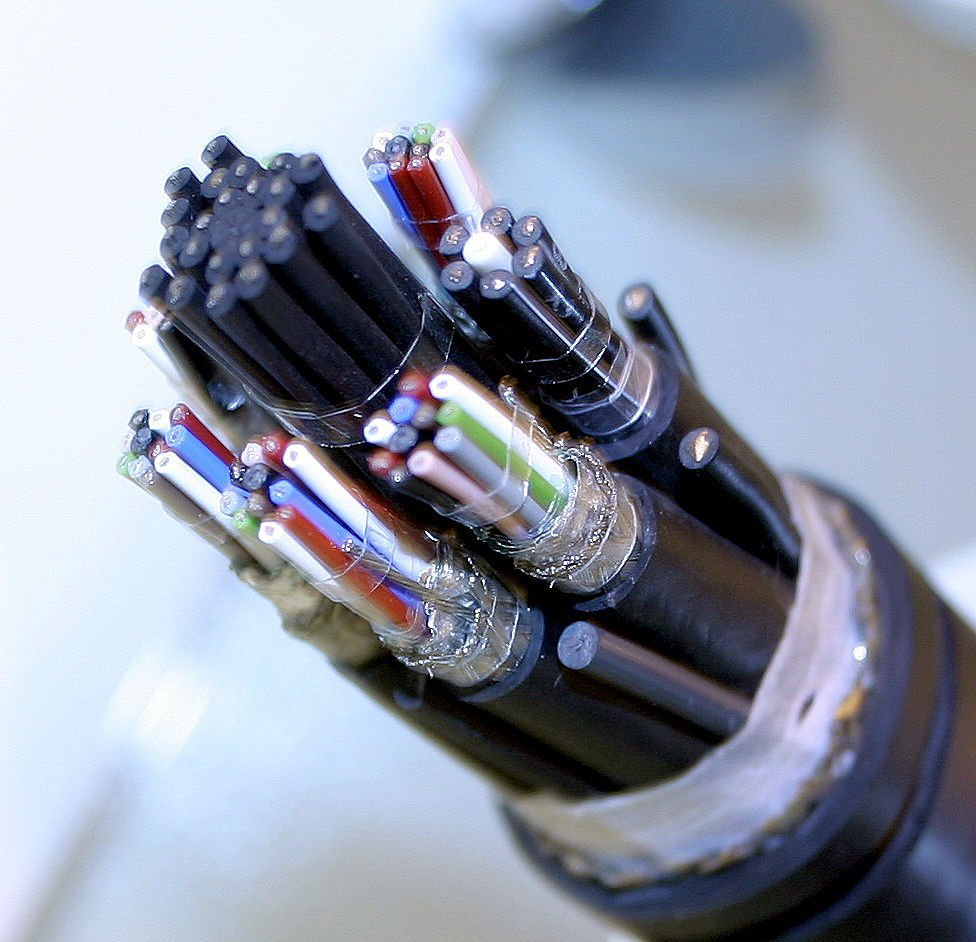
\includegraphics[height=0.4\textheight]{\resdir/cablesm.jpg}

	\begin{block}<+-> {C�ble}
		\begin{itemize}
		\item Diff�rentes caract�ristiques
			\begin{itemize}
			\item Att�nuation
			\item Bande-passante
			\item Vitesse de propagation
			\item Prix
			\end{itemize}
		\item Couche OSI 1 
		\end{itemize}	
	\end{block}
	
\end{frame}
% ----------------------------------------------------------------------

% ----------------------------------------------------------------------
\begin{frame}

\centering
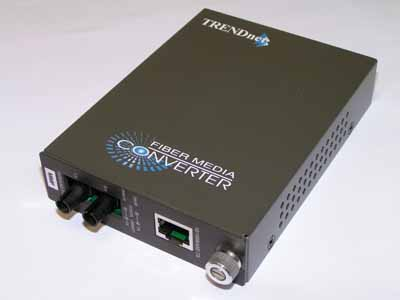
\includegraphics[height=\imgheight]{\resdir/repeteur.jpg}

	\begin{block}<+-> {R�p�teur (\textit{repeater})}
		\begin{itemize}
		\item Reg�n�re le signal entre deux c�bles
		\item Pour d�passer les limites d'att�nuation
		\item R�p�te sur un port ce qu'il entend sur l'autre
		\item Couche OSI 1
		\end{itemize}	
	\end{block}
	
\end{frame}
% ----------------------------------------------------------------------

% ----------------------------------------------------------------------
\subsection{Mat�riel interne}
% ----------------------------------------------------------------------
\begin{frame}

\centering
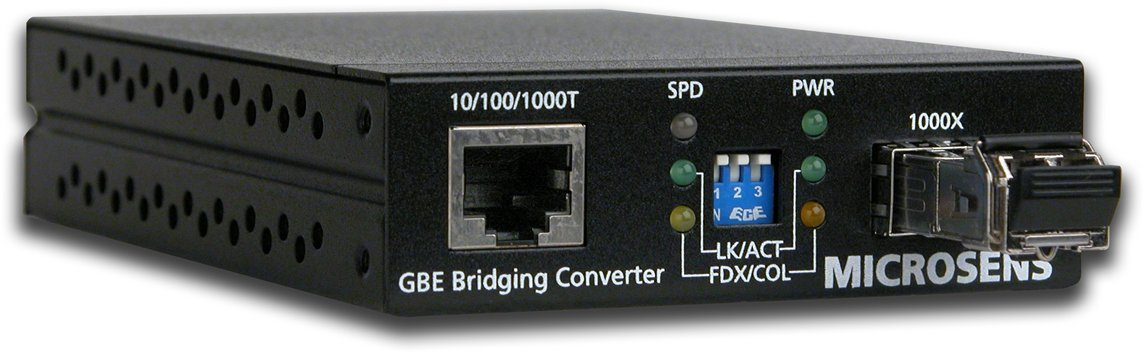
\includegraphics[width=\textwidth]{\resdir/pont.jpg}

	\begin{block}<+-> {Pont (\textit{bridge})}
		\begin{itemize}
		\item Relie des r�seau travaillant avec le m�me protocole
		\item = Filtre les trames � destination du r�seau de l'autre c�t�
		\item Permet de segmenter le r�seau (r�duction du trafic)
		\item Couche OSI 1 et 2 (adresse MAC)
		\end{itemize}	
	\end{block}
	
\end{frame}
% ----------------------------------------------------------------------

% ----------------------------------------------------------------------
\begin{frame}

\centering
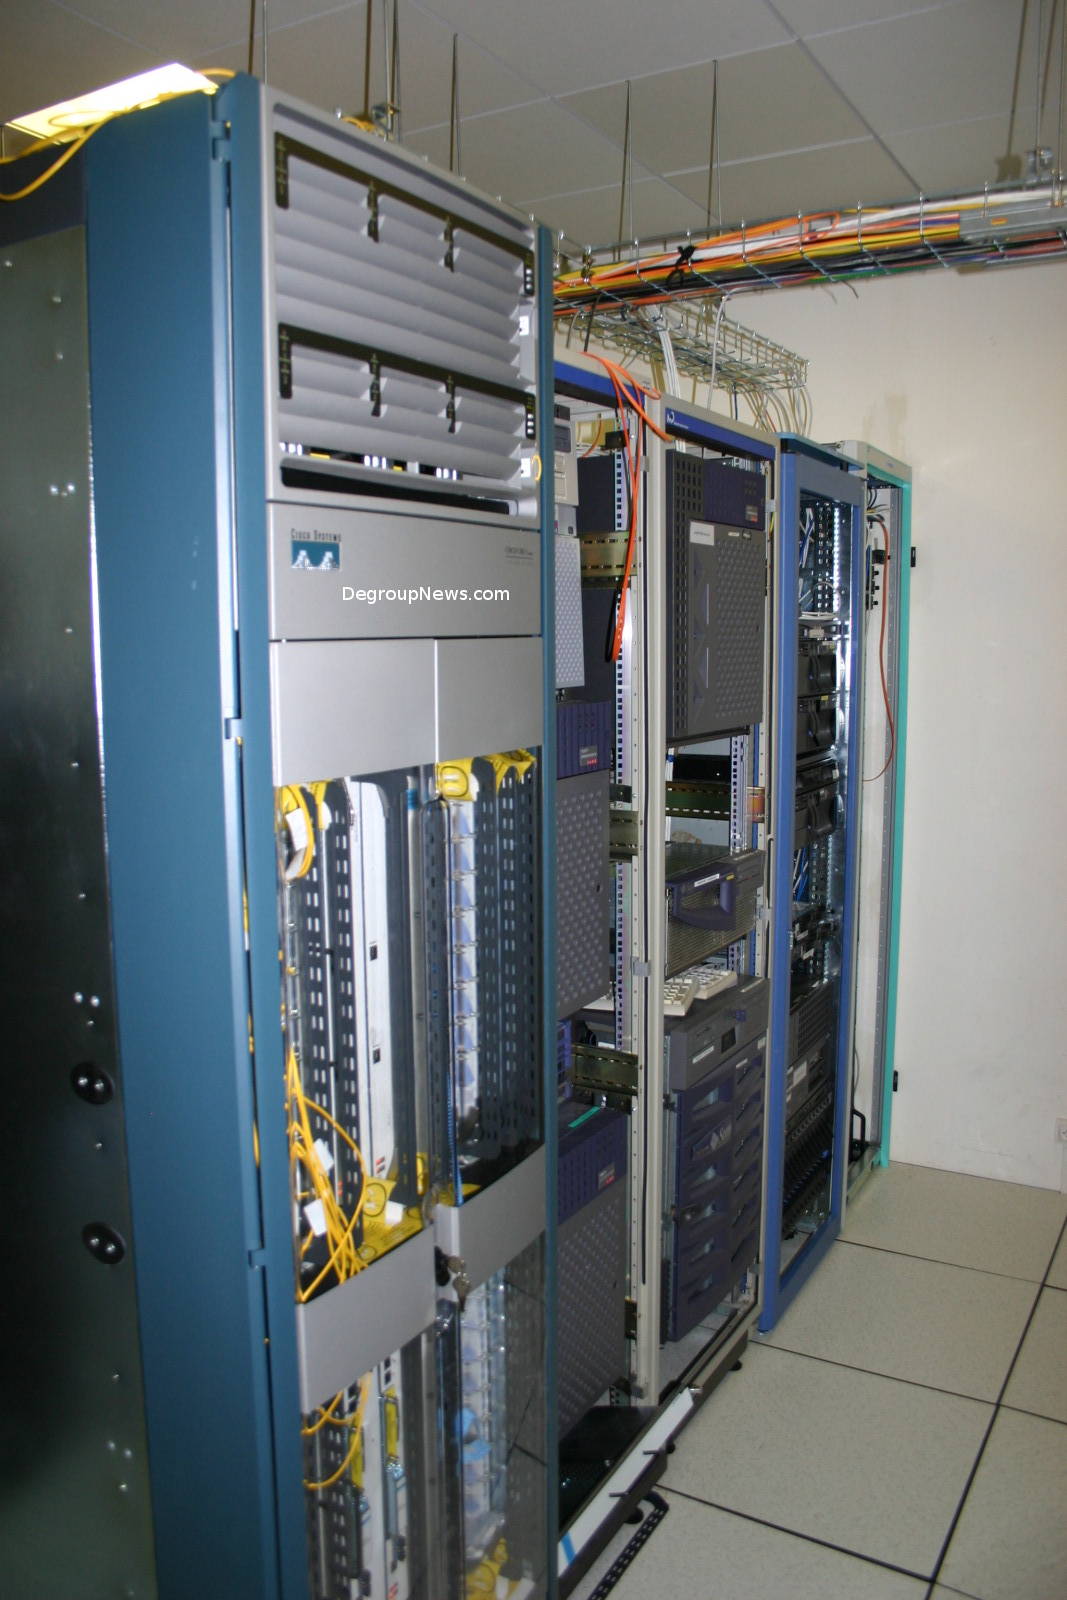
\includegraphics[height=0.5\textheight]{\resdir/routeur.jpg}

	\begin{block}<+-> {Routeur (\textit{router})}
		\begin{itemize}
		\item Route les paquets entre les diff�rents r�seaux
		\item Interne � l'internet
		\item D�termine le chemin � emprunter (table de routage)
		\item Impl�mente un algorithme de routage
		\end{itemize}	
	\end{block}
	
\end{frame}
% ----------------------------------------------------------------------


% ----------------------------------------------------------------------
\begin{frame}

\centering
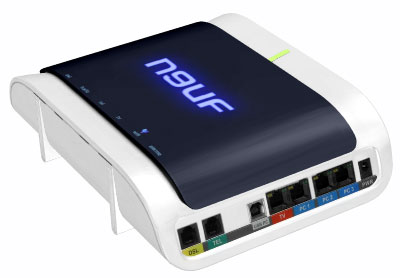
\includegraphics[width=0.32\textwidth]{\resdir/neufbox.jpg}\hfill
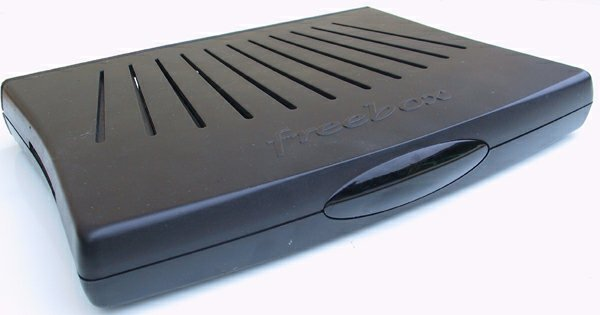
\includegraphics[width=0.32\textwidth]{\resdir/freebox.jpg}\hfill
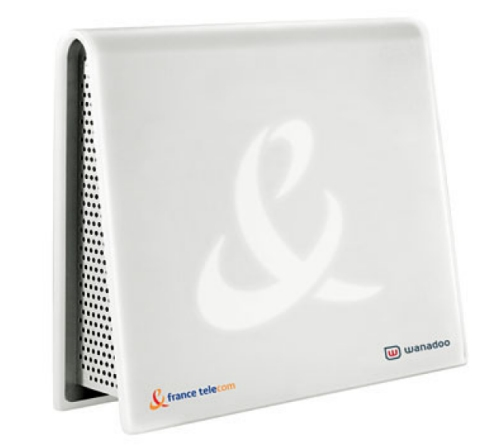
\includegraphics[width=0.32\textwidth]{\resdir/livebox.jpg}

	\begin{block}<+-> {Passerelle (\textit{gateway})}
		\begin{itemize}
		\item Pont entre deux r�seaux de protocole diff�rents
		\item Mat�riel et logiciel
		\item Exemple : modem ou tunnel (VPN)
		\end{itemize}	
	\end{block}
	
\end{frame}
% ----------------------------------------------------------------------


% ----------------------------------------------------------------------
\begin{frame}

\centering
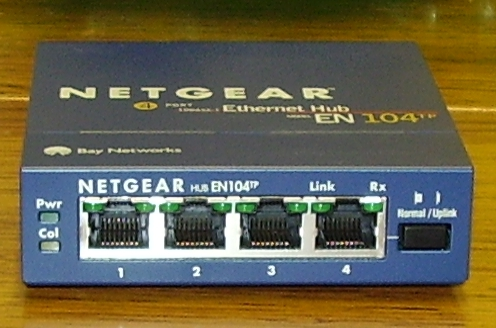
\includegraphics[height=\imgheight]{\resdir/concentrateur}

	\begin{block}<+-> {Concentrateur (\textit{hub})}
		\begin{itemize}
		\item Concentre le trafic de plusieurs h�tes
		\item Rediffusion du trafic arrivant sur chaque port sur tous les autres
		\item \'Egalement : r�p�teur
		\item 4/8/16/32 ports
		\item Couche OSI 1 
		\item Actif (aliment�) ou passif
		\item Connectable en cascade (port uplink/c�ble crois�)
		\end{itemize}	
	\end{block}
	
\end{frame}
% ----------------------------------------------------------------------


% ----------------------------------------------------------------------
\begin{frame}

\centering
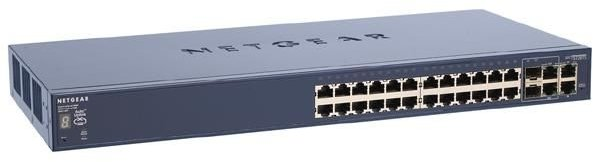
\includegraphics[width=\textwidth]{\resdir/commutateur.jpg}

	\begin{block}<+-> {Commutateur (\textit{switch})}
		\begin{itemize}
		\item Pont multiports
		\item Concentre et redirige les donn�es vers la bonne destination
		\item 4-96 ports		
		\item Couche OSI 1 et 2
		\item \'Egalement : commutateur de niveau 7
		\end{itemize}	
	\end{block}
	
\end{frame}
% ----------------------------------------------------------------------


% ----------------------------------------------------------------------
\begin{frame}

\centering
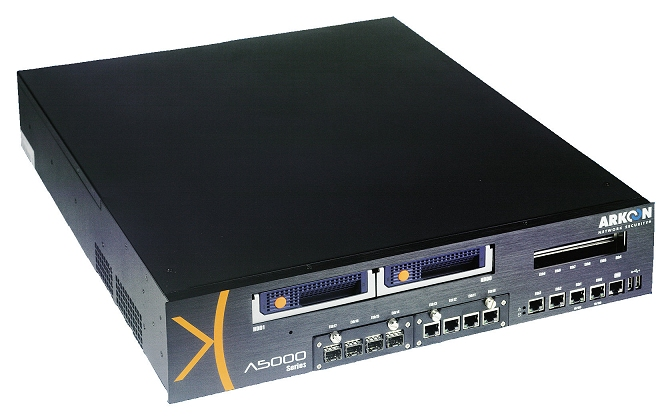
\includegraphics[height=\imgheight]{\resdir/parefeu.jpg}

	\begin{block}<+-> {Pare-feu (\textit{firewall})}
		\begin{itemize}
		\item Filtre les communications (s�curit�)
		\item Mat�riel ou logiciel
		\item R�seau (par port/protocole) ou applicatif (par application/port/protocole)
		\item Analyse plus ou moins profonde des communications
		\item Gestion dynamique des ports
		\item Permet aussi de faire des translations (NAT/PAT)
		\end{itemize}	
	\end{block}
	
\end{frame}
% ----------------------------------------------------------------------

% ----------------------------------------------------------------------
\subsection{Mat�riel d'extr�mit�}
%TODO : ajouter smartphone, pc
% ----------------------------------------------------------------------
\begin{frame}

\centering
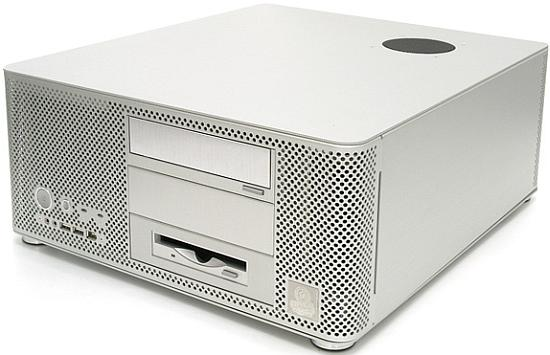
\includegraphics[height=\imgheight]{\resdir/PC.jpg}

	\begin{block}<+-> {Serveur mandataire (\textit{proxy server})}
		\begin{itemize}
		\item Masque les machines \og derri�re\fg
		\item Filtrage
		\item Authentification
		\item Cache
		\item Machine classique
		\end{itemize}	
	\end{block}
	
\end{frame}
% ----------------------------------------------------------------------


% ----------------------------------------------------------------------
\begin{frame}

\centering
\only<1>{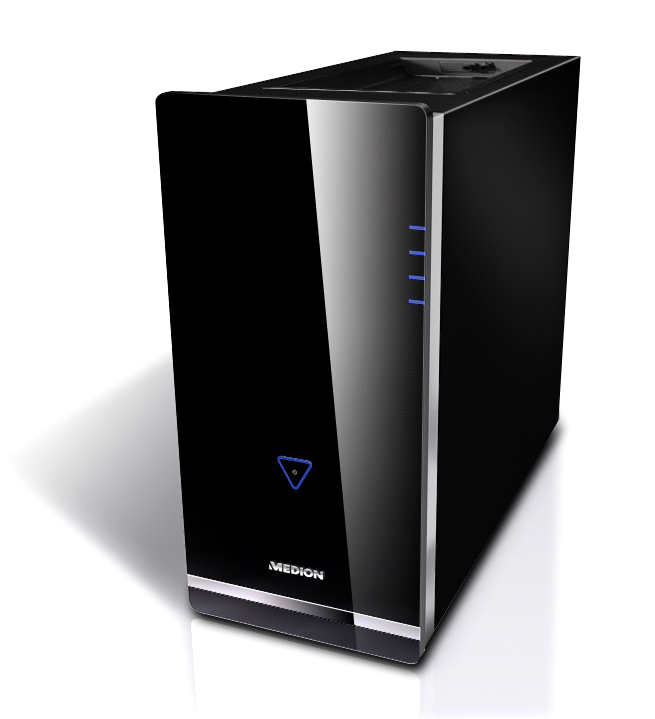
\includegraphics[height=\imgheight]{\resdir/serveur-home.jpg} \hspace{2cm} 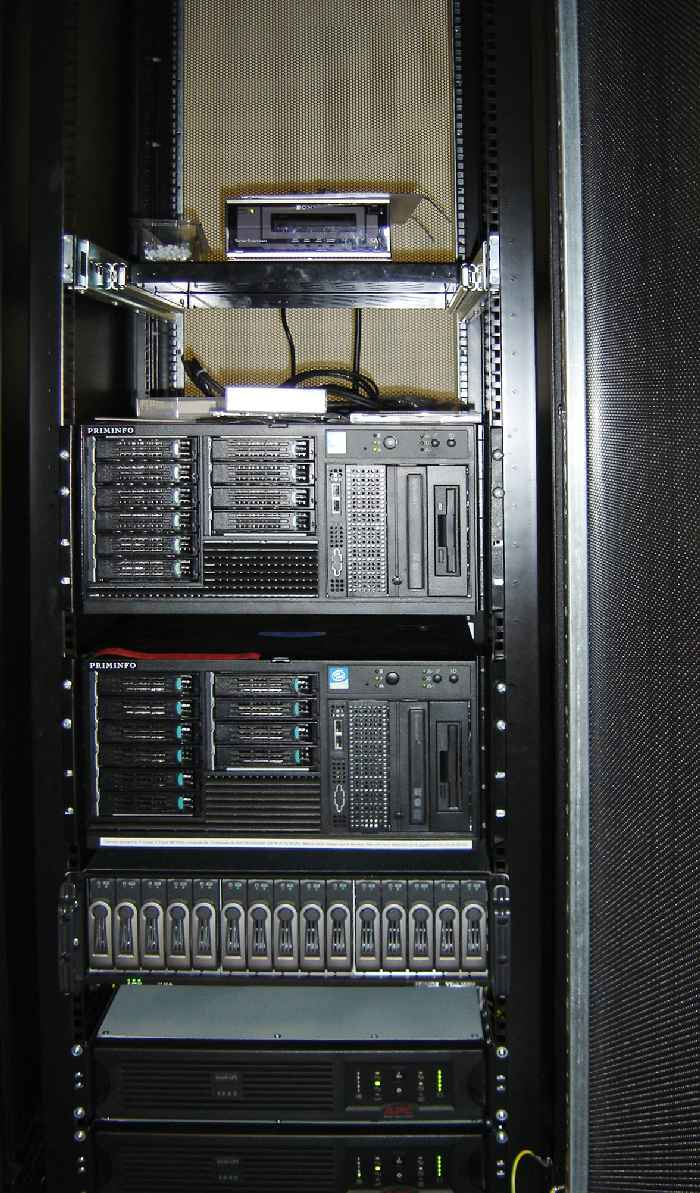
\includegraphics[height=\imgheight]{\resdir/serveur-armoire.jpg}}
\only<2>{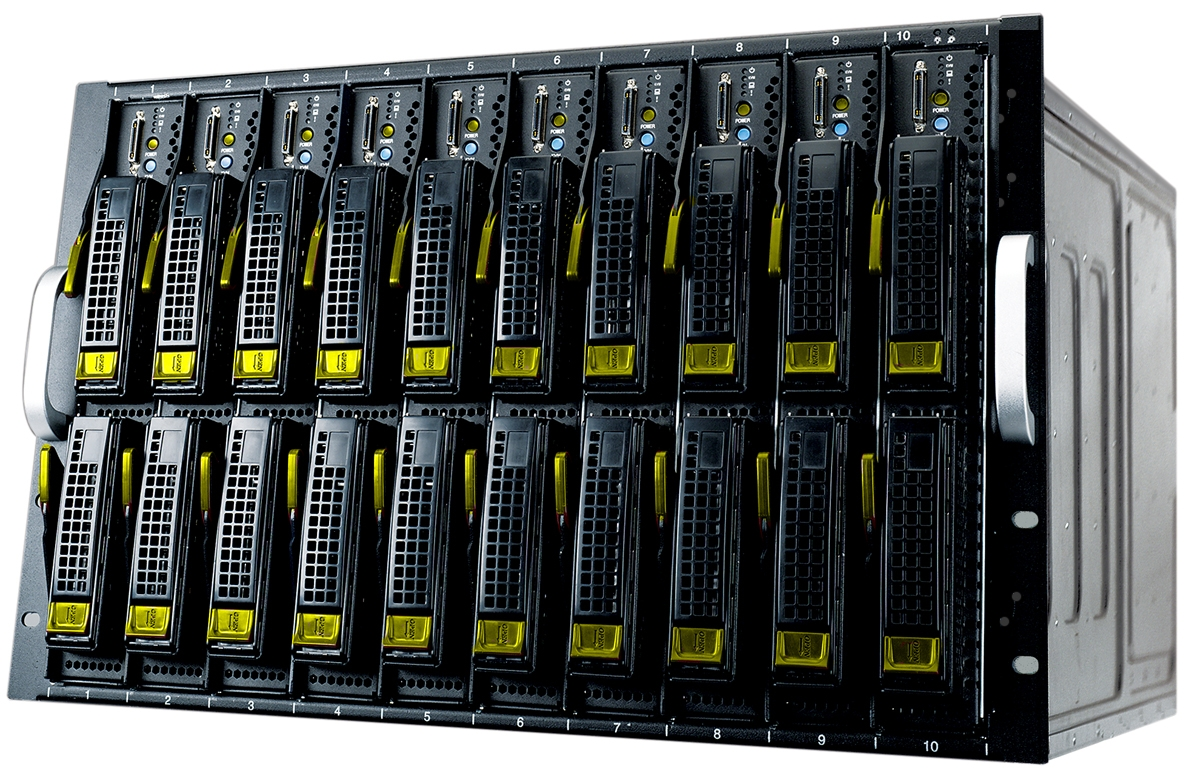
\includegraphics[height=\imgheight]{\resdir/serveur-blade.jpg}
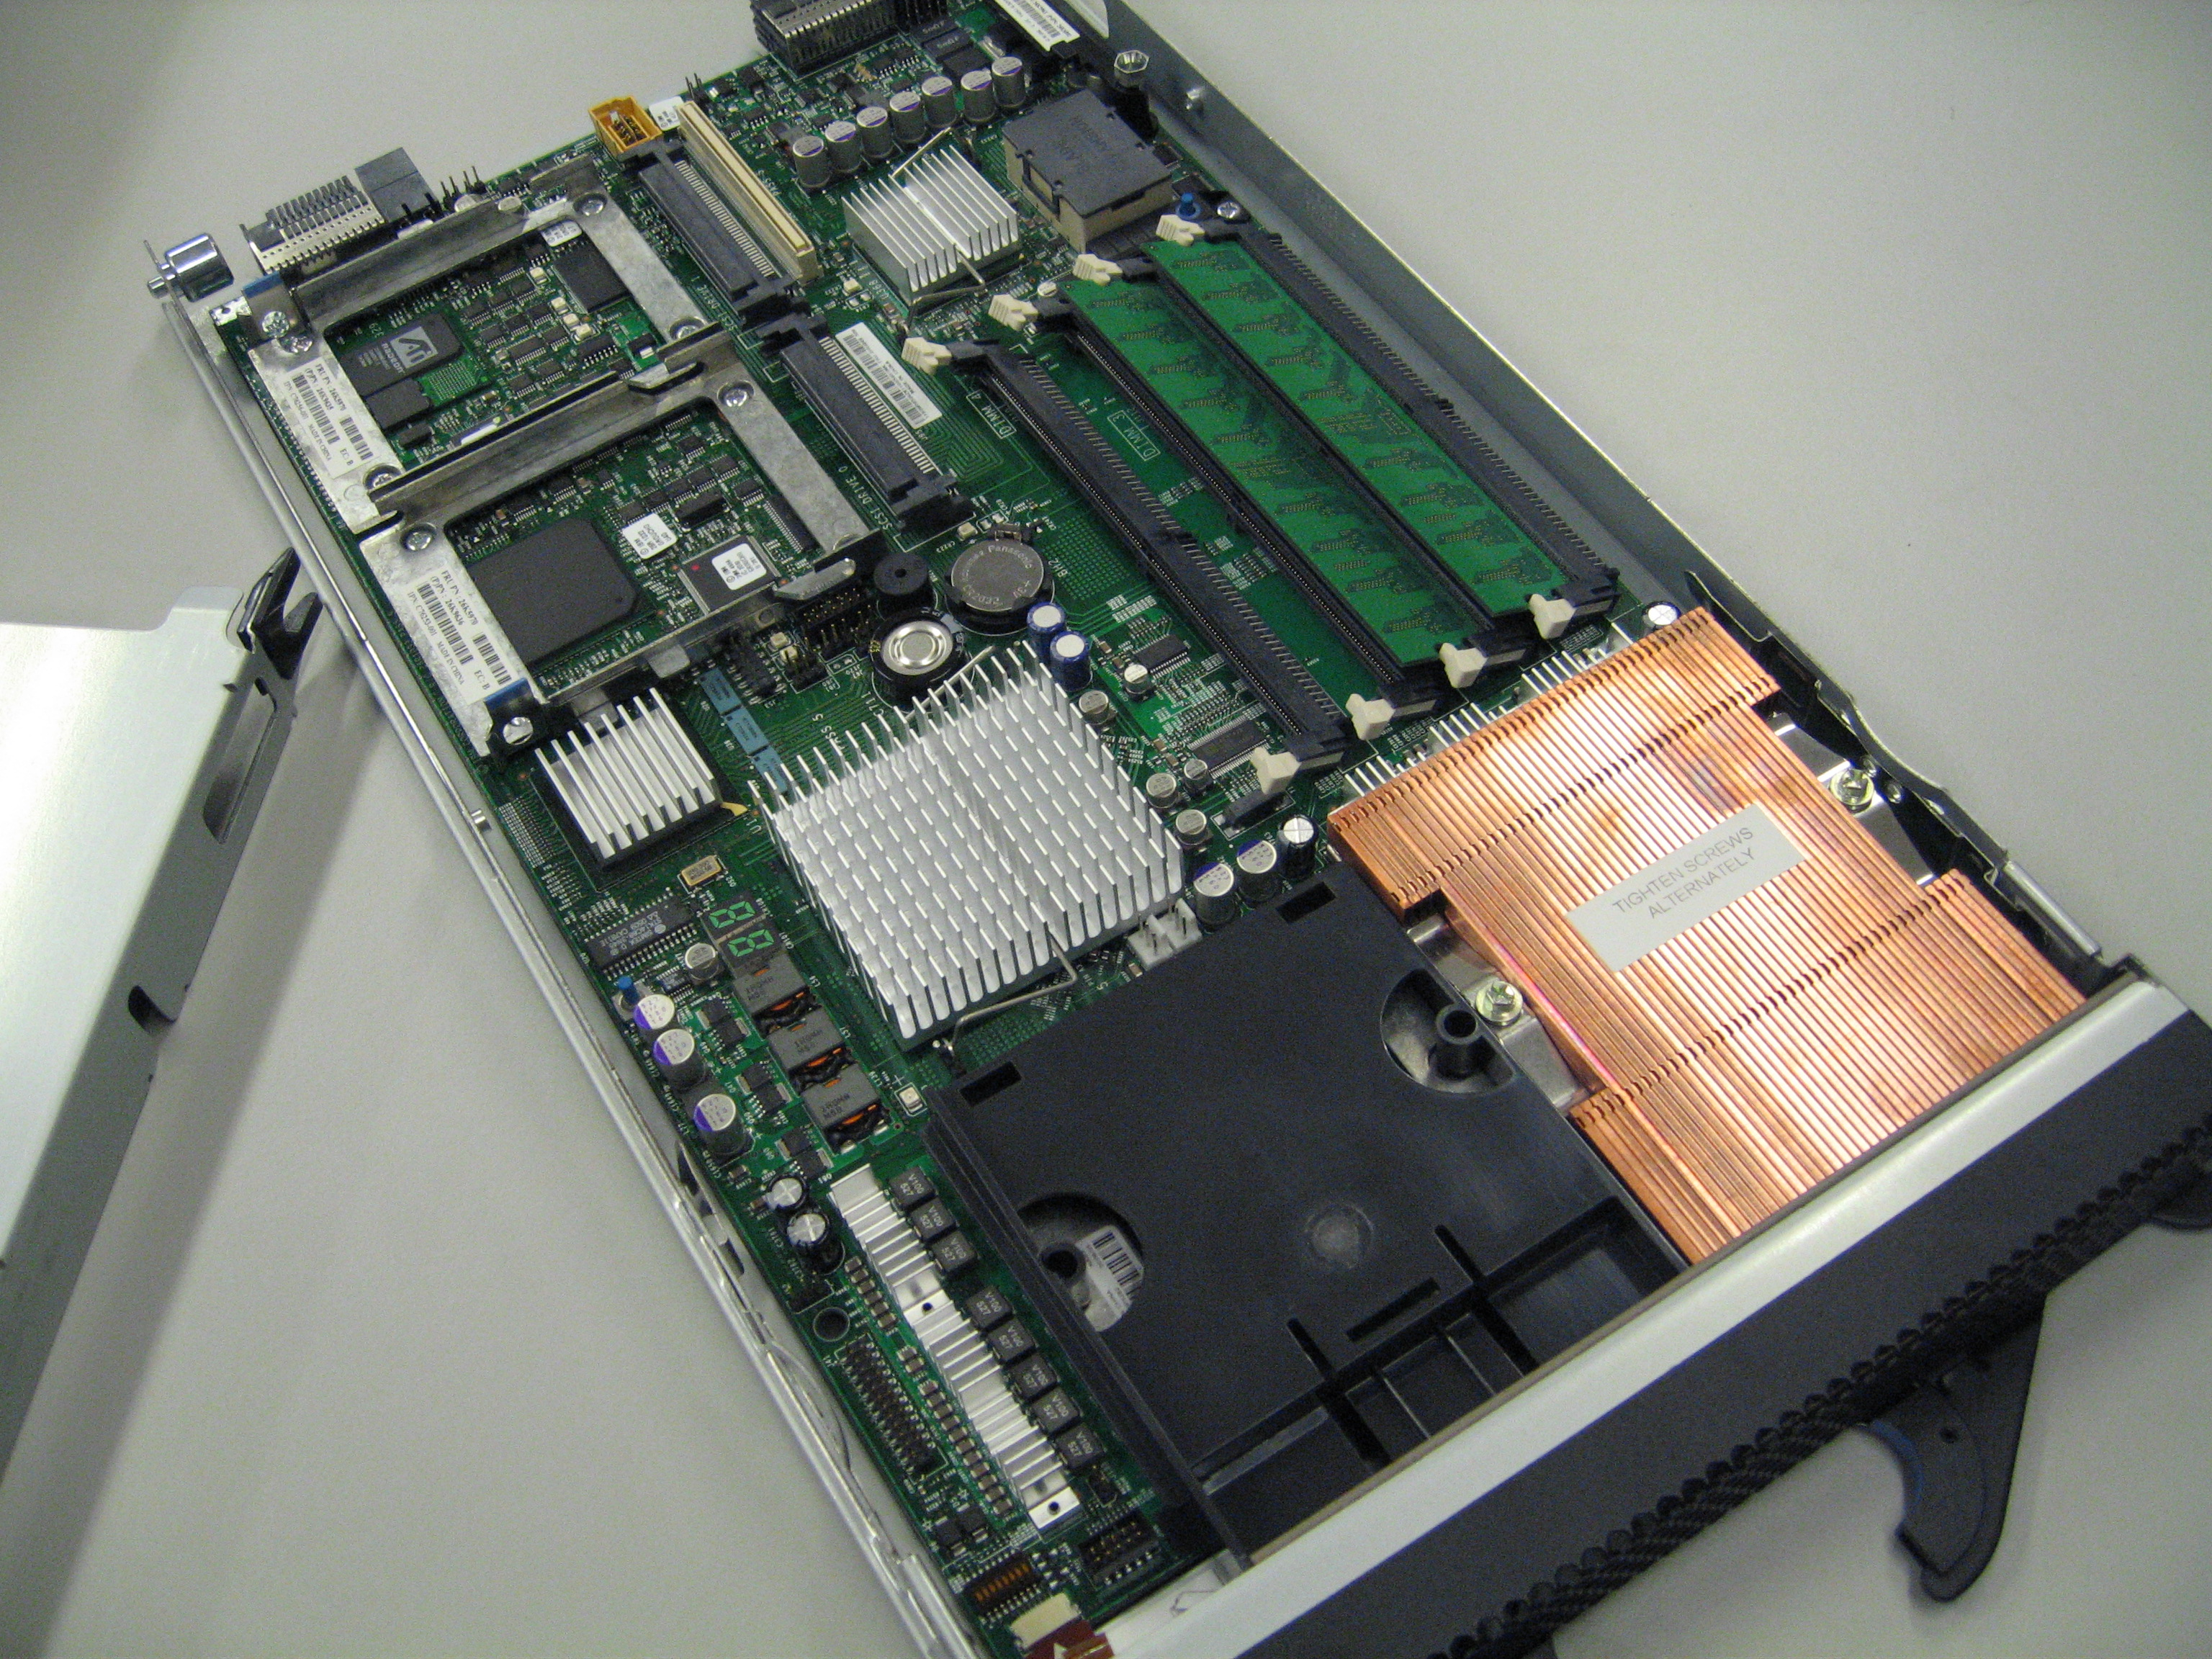
\includegraphics[height=\imgheight]{\resdir/blade.jpg}}
\only<3>{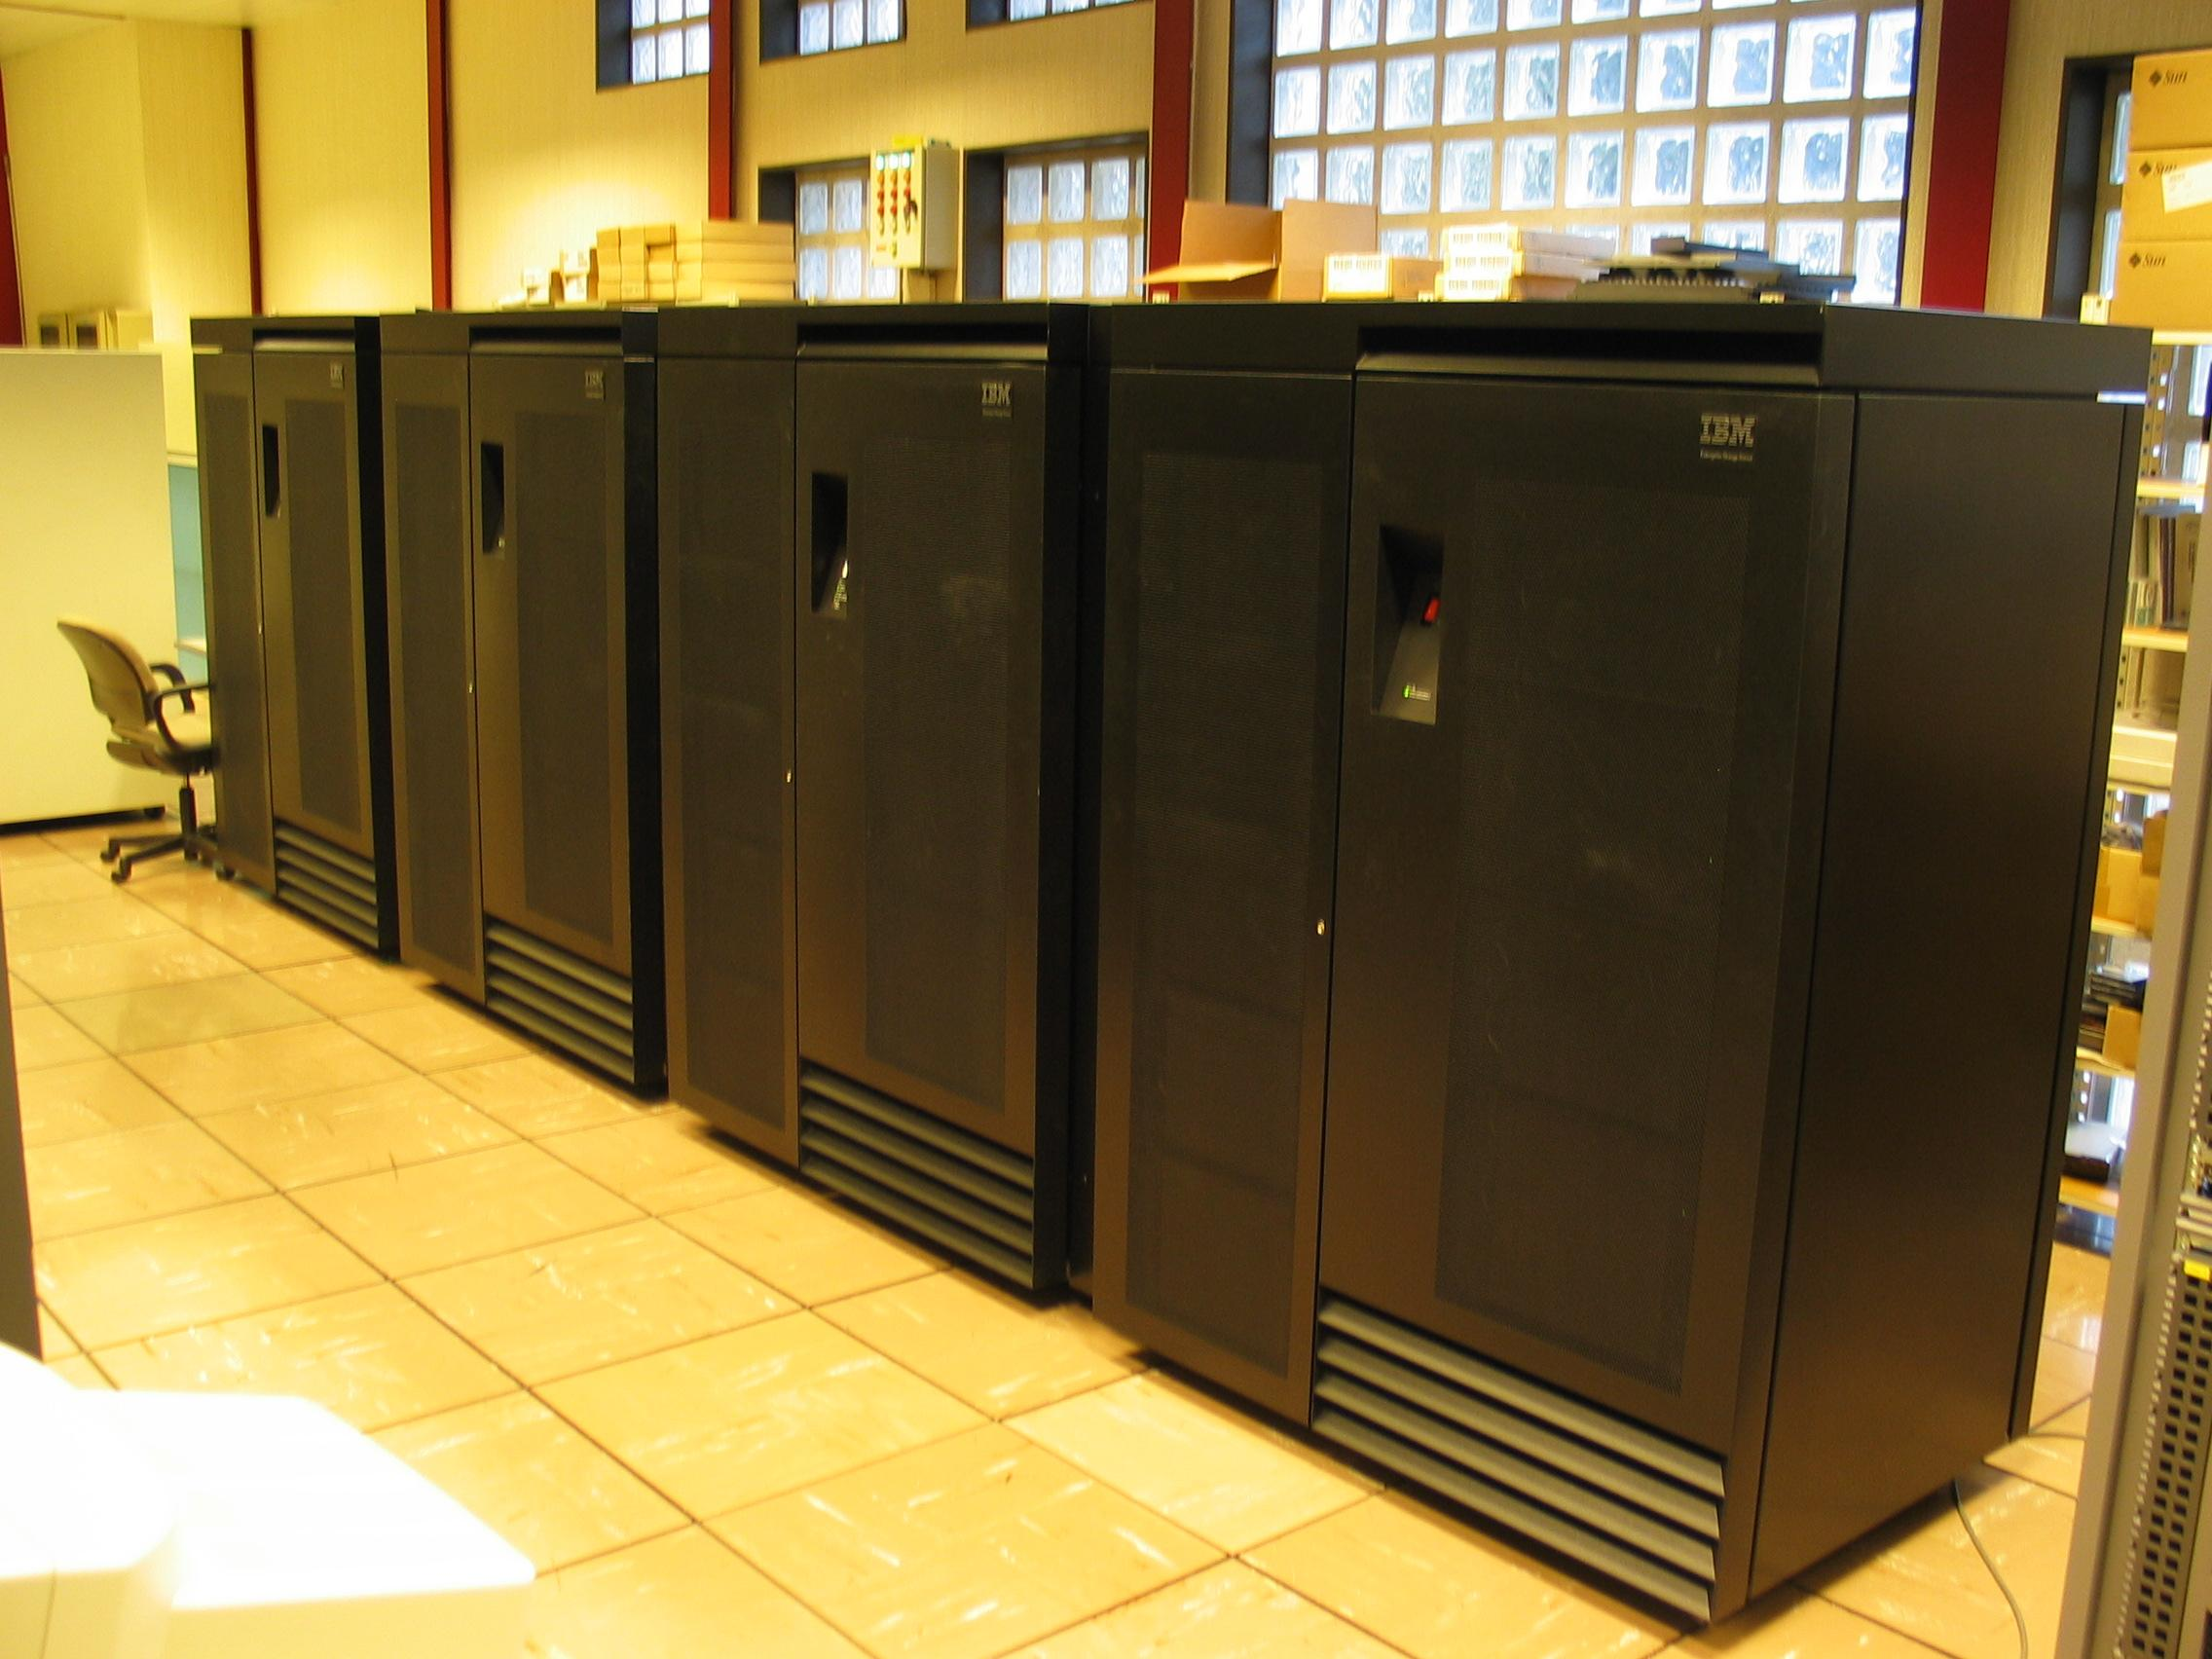
\includegraphics[height=\imgheight]{\resdir/serveur-fichier.jpg}}

	\begin{block}<+-> {Serveur (\textit{server})}
		\begin{itemize}
		\item Ex�cute les applications
		\item Mat�riel ET logiciel
		\item Plus ou moins performant
			\begin{itemize}
				\item CPU, m�moire, disque, communication
			\end{itemize}
		\item Louable
			\begin{itemize}
				\item stockage, h�bergement Web ou pas, calcul, jeu\ldots
			\end{itemize}
		\item Mode actuelle : externalisation et virtualisation
		\end{itemize}	
	\end{block}
	
\end{frame}
% ----------------------------------------------------------------------

% ----------------------------------------------------------------------
\begin{frame}

\centering
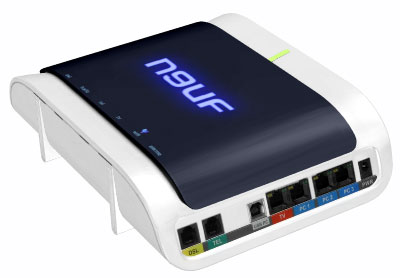
\includegraphics[width=0.32\textwidth]{\resdir/neufbox.jpg}\hfill
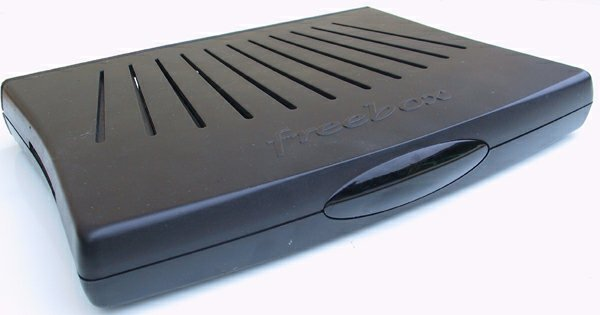
\includegraphics[width=0.32\textwidth]{\resdir/freebox.jpg}\hfill
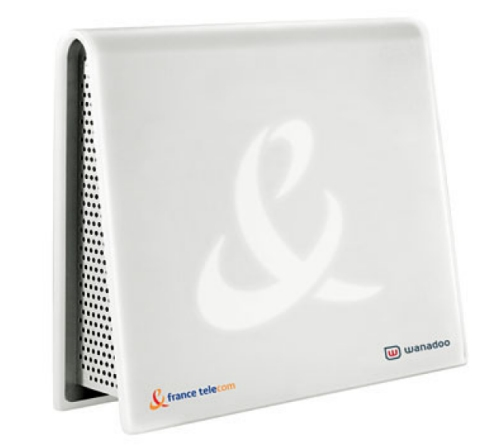
\includegraphics[width=0.32\textwidth]{\resdir/livebox.jpg}

	\begin{block}<+-> {adslbox}
		\begin{itemize}
		\item Pont + Passerelle + Proxy
		\item Switch
		\item Proxy
		\item Routeur (un peu)
		\item Parefeu
		\item Hotspot wifi (priv� et public)
		\item Serveur : DHCP, FTP, impression\ldots
		\end{itemize}	
	\end{block}
	
\end{frame}
% ----------------------------------------------------------------------

%
%\def\resdir{3protocoles}

% ----------------------------------------------------------------------
\section{Protocoles}
% ----------------------------------------------------------------------


% ----------------------------------------------------------------------
\begin{frame}

\centering
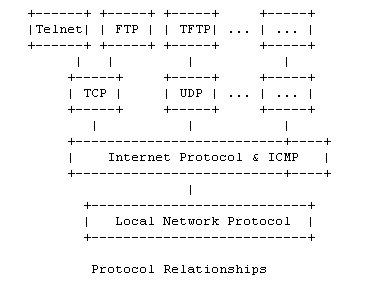
\includegraphics[width=\textwidth]{\resdir/protocol_relationship.jpg}

\end{frame}
% ----------------------------------------------------------------------




% ----------------------------------------------------------------------
\subsection{Local Network Protocol}
% ----------------------------------------------------------------------

% ----------------------------------------------------------------------
\begin{frame}{Local Network Protocol}

	\begin{block}<+-> {R�seaux avant Internet}
	\begin{itemize}
		\item Local = Non-�tendu
		\item \`A l'origine : \textit{ALOHAnet}
		\item Un seul m�dia de communication
		\item Protocole principal : \textit{Ethernet}
	\end{itemize}					
	\end{block}
		
\end{frame}
% ----------------------------------------------------------------------

% ----------------------------------------------------------------------
\begin{frame}

	\centering
	
	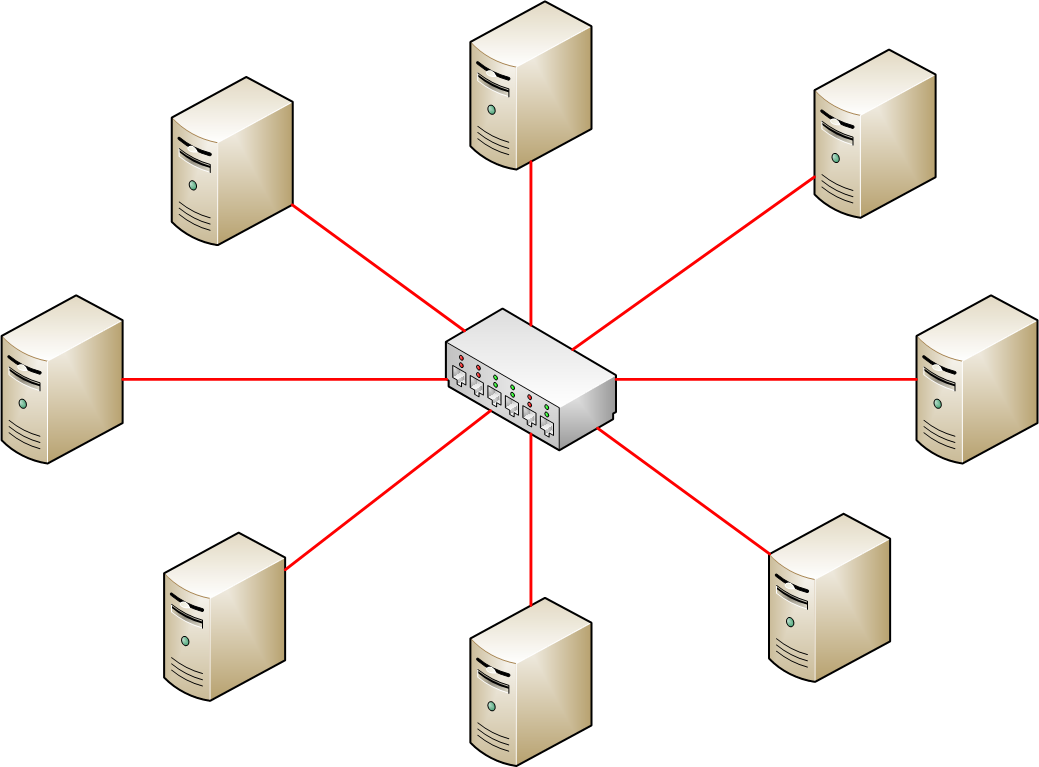
\includegraphics[height=0.6\textheight]{\resdir/ethernet}
	
	\begin{block}<+-> {Topologie}
		\begin{itemize}
			\item En \'Etoile
			\item Autour d'un hub ou d'un switch
		\end{itemize}
	\end{block}
	
\end{frame}
% ----------------------------------------------------------------------

% ----------------------------------------------------------------------
\begin{frame}
	\begin{columns}
	
	\column{0.5\textwidth}
		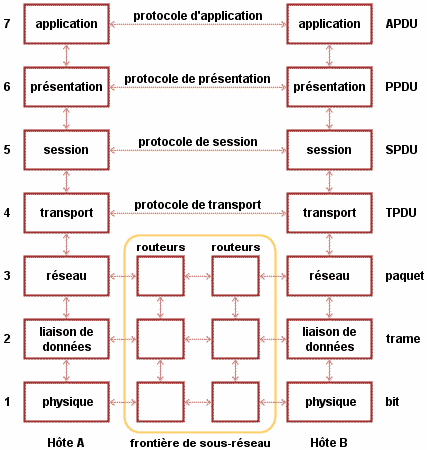
\includegraphics[height=0.8\textheight]{\resdir/osi}
	
	\column{0.5\textwidth}
		\begin{block}<+-> {Ethernet}
			\begin{itemize}
			\item Protocole R�seau local
			\item Unique ligne de communication
				\item Impl�mentation des couches
				\begin{itemize}
					\item Liaison
					\item Physique
				\end{itemize}
				\item Ether - Net(work)
				\item Bas� sur l'adresse MAC
				\begin{itemize}
					\item Media Access Control 
				\end{itemize}
				\item \'Echange de \textit{Trames}
				\item 10 Mb/s � 10 Gb/s
			\end{itemize}
		\end{block}
		
	\end{columns}		
\end{frame}
% ----------------------------------------------------------------------






% ----------------------------------------------------------------------
\subsection{Internet}
% ----------------------------------------------------------------------


% ----------------------------------------------------------------------
\begin{frame}{Inter-Network Protocols}

	\begin{block}<+-> {Deux niveaux g�n�riques basiques}
	\begin{itemize}
		\item R�seau Local : Ethernet
		\item R�seau Global : Internet
			\begin{itemize}
			\item IP : Internet Protocol
			\item ICMP : Internet Control Message Protocol
			\item GGP : Gateway to Gateway Protocol
			\end{itemize}
		\end{itemize}					
		\end{block}
		
		\centering
		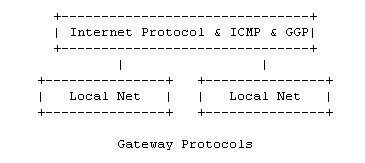
\includegraphics[width=\textwidth]{\resdir/gateways_protocol.jpg}

\end{frame}
% ----------------------------------------------------------------------

% ----------------------------------------------------------------------
\begin{frame}{Internet}

	\centering
	
	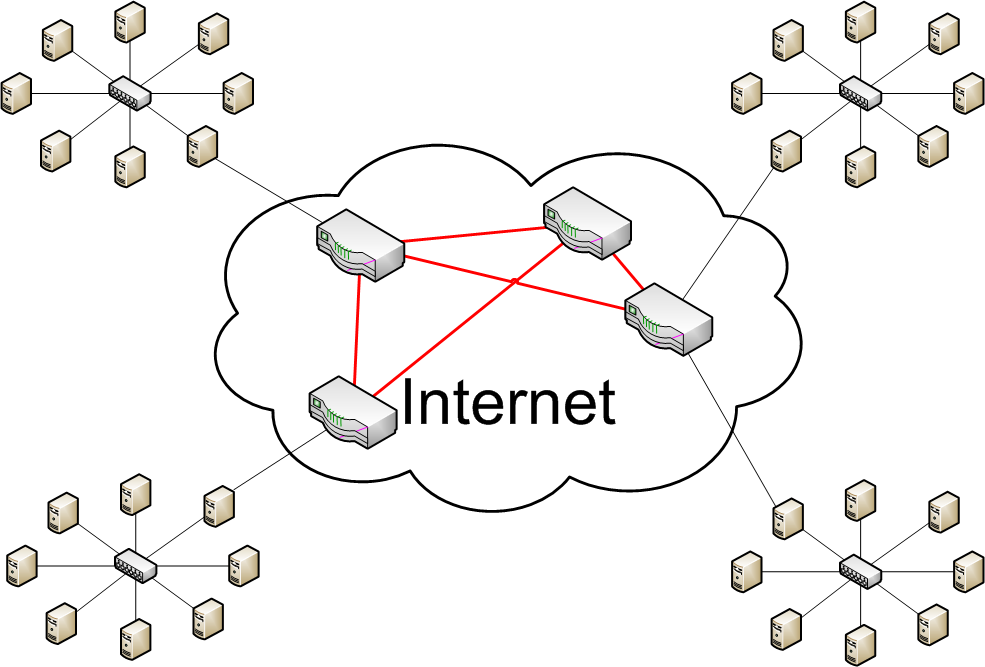
\includegraphics[height=0.6\textheight]{\resdir/internet}
	
	\begin{block}<+-> {Topologie}
		\begin{itemize}
			\item Quelconque
			\item R�seaux locaux en ``bordure''
			\item Inter-Net(work)
		\end{itemize}
	\end{block}
	
\end{frame}
% ----------------------------------------------------------------------


% ----------------------------------------------------------------------
\begin{frame}
	\begin{columns}
	
	\column{0.5\textwidth}
		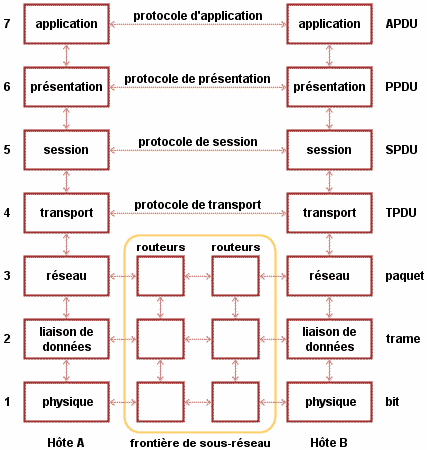
\includegraphics[height=0.8\textheight]{\resdir/osi}
	
	\column{0.5\textwidth}
		\begin{block}<+-> {IP : Internet Protocol}
			\begin{itemize}
			\item Protocole R�seau de R�seaux
			\item D�crit dans la RFC 791							
			\item Rout�
			\item Impl�mentation de la couche
				\begin{itemize}
					\item R�seau
				\end{itemize}
				\item Bas� sur l'adresse IP
				\begin{itemize}
					\item IPv4 ou IPv6
				\end{itemize}
				\item \'Echange de \textit{Paquets}
				\item Ne g�re pas les erreurs
			\end{itemize}
		\end{block}
		
	\end{columns}		
\end{frame}
% ----------------------------------------------------------------------

% ----------------------------------------------------------------------
\begin{frame}

	\centering
	
	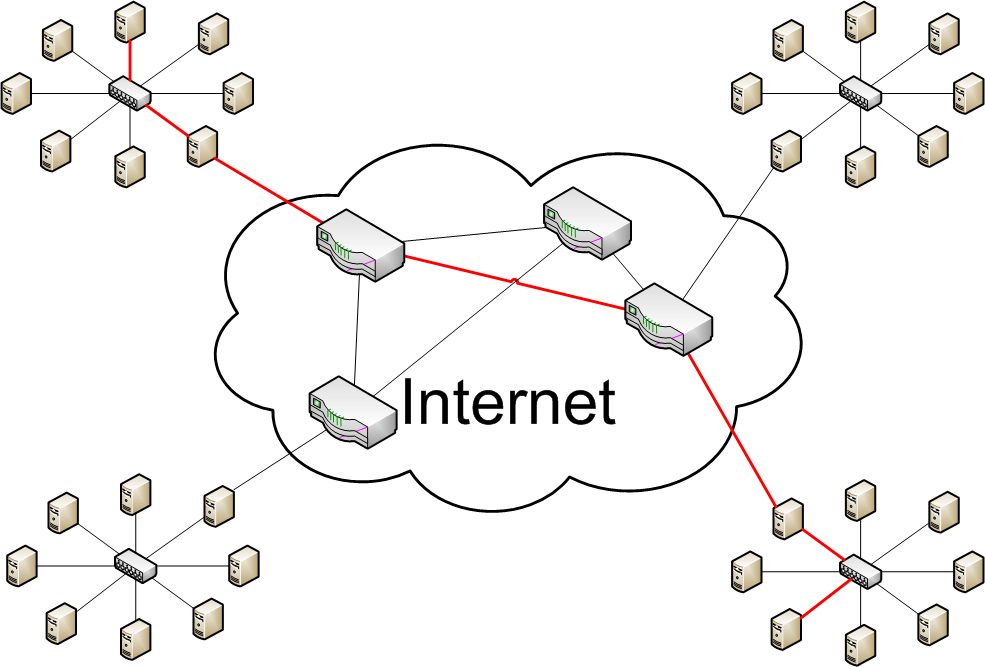
\includegraphics[height=0.6\textheight]{\resdir/bout-en-bout}
	
	\begin{block}<+-> {Communications de Bout-en-Bout}
		\begin{itemize}
			\item Entre deux machines terminales
		\end{itemize}
	\end{block}
	
\end{frame}
% ----------------------------------------------------------------------



% ----------------------------------------------------------------------
\begin{frame}
	\begin{columns}
	
	\column{0.5\textwidth}
		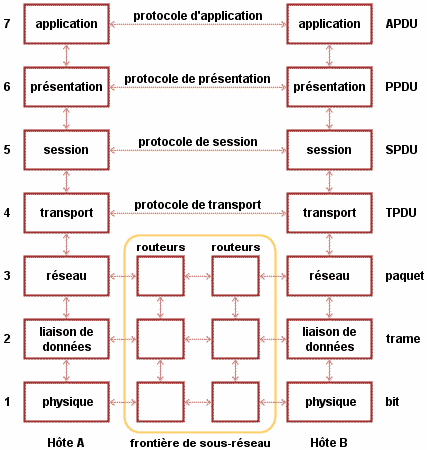
\includegraphics[height=0.8\textheight]{\resdir/osi}
	
	\column{0.5\textwidth}
		\begin{block}<+-> {ICMP : Internet Control Message Protocol}
			\begin{itemize}
			\item Protocole R�seau de R�seaux
			\item D�crit dans la RFC 792							
			\item Rout�
			\item Agit au niveau de la couche
				\begin{itemize}
				\item R�seau
				\end{itemize}
			\item G�re les erreurs et l'administration
				\begin{itemize}
				\item P.ex. msg (echo) pour ping
				\end{itemize}
			\end{itemize}
		\end{block}
		
	\end{columns}		
\end{frame}
% ----------------------------------------------------------------------

% ----------------------------------------------------------------------
\begin{frame}
	\begin{columns}
	
	\column{0.5\textwidth}
		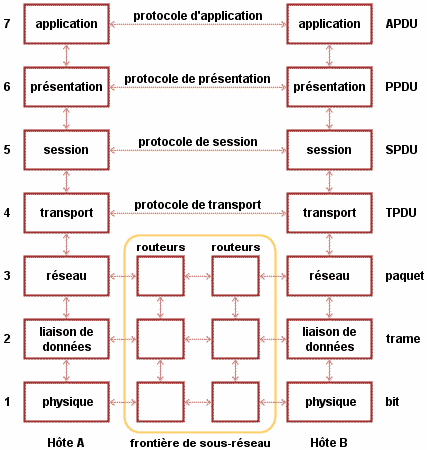
\includegraphics[height=0.8\textheight]{\resdir/osi}
	
	\column{0.5\textwidth}
		\begin{block}<+-> {GGP : Gateway to Gateway Protocol}
			\begin{itemize}
			\item Obsol�te : BGP Border Gateway Protocol
			\item D�crit dans la RFC 4271		
			\item Agit au niveau de la couche
				\begin{itemize}
				\item R�seau
				\end{itemize}
			\item MAJ des routes entre routeurs
				\begin{itemize}
				\item Entre Autonomous Systems (AS)
				\end{itemize}
			\end{itemize}
		\end{block}

	\end{columns}
\end{frame}
% ----------------------------------------------------------------------




% ----------------------------------------------------------------------
\subsection{Protocoles de Communication Applicatives}
% ----------------------------------------------------------------------



% ----------------------------------------------------------------------
\begin{frame}{Protocoles de Communication Applicatives}

\centering
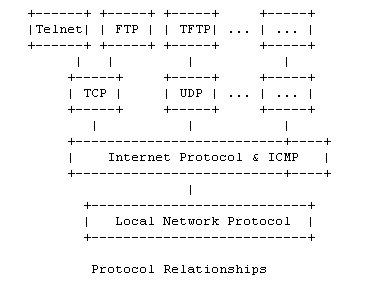
\includegraphics[width=0.8\textwidth]{\resdir/protocol_relationship.jpg}

\end{frame}
% ----------------------------------------------------------------------


% ----------------------------------------------------------------------
\begin{frame}{Protocoles de Communication Applicatives G�n�riques}

	\centering
	
	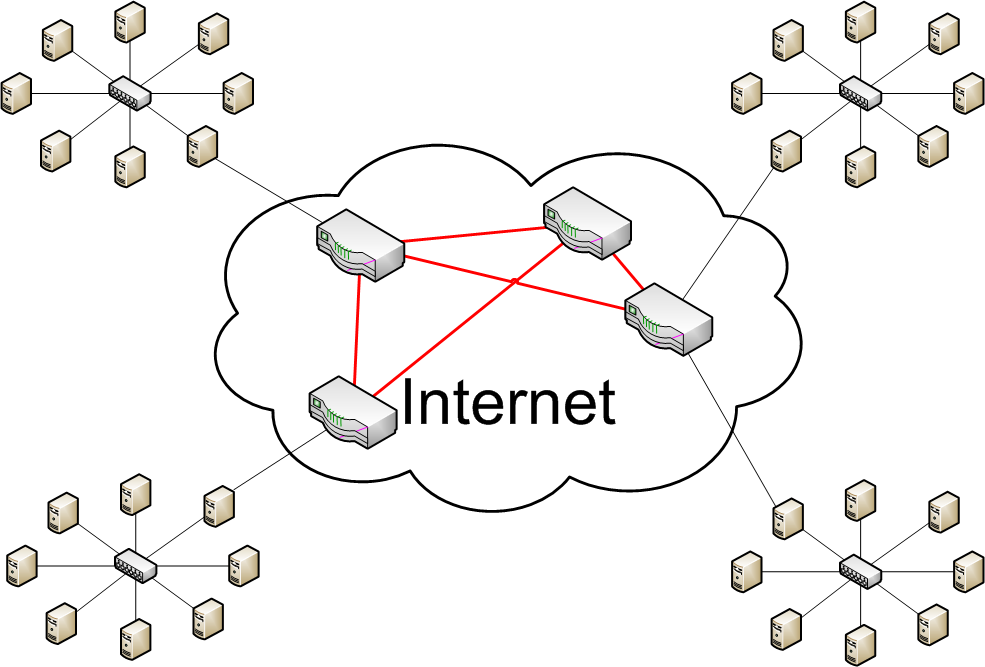
\includegraphics[height=0.4\textheight]{\resdir/internet}
	
	\begin{block}<+-> {Communications de Bout-en-Bout}
		\begin{itemize}
			\item Entre deux applications
			\item Gr�ce � la notion de \textit{port}
			\item Deux protocoles principaux
				\begin{itemize}
				\item TCP : Transmission Control Protocol (connect�)
				\item UDP : User Datagram Protocol  (d�connect�)
				\end{itemize}
		\end{itemize}
	\end{block}
	
\end{frame}
% ----------------------------------------------------------------------

% ----------------------------------------------------------------------
\begin{frame}
	\begin{columns}

	\column{0.5\textwidth}
		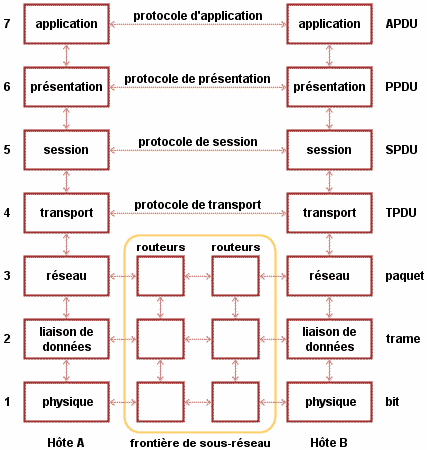
\includegraphics[height=0.8\textheight]{\resdir/osi}

	\column{0.5\textwidth}
		\begin{block}<+-> {TCP/UDP}
			\begin{itemize}
			\item Protocole Port � Port
			\item D�crits dans les RFC 793/768						
			\item Impl�mente la couche
				\begin{itemize}
				\item Transport (4)
				\item Session pur TCP (5)
				\end{itemize}
			\item Transporte l'information
				\begin{itemize}
				\item Entre deux applications
				\item Plus ou moins de services
				\end{itemize}
			\end{itemize}
		\end{block}

	\end{columns}		
\end{frame}
% ----------------------------------------------------------------------




% ----------------------------------------------------------------------
\begin{frame}{Protocoles de Communication Applicatives Sp�cifiques}

\centering
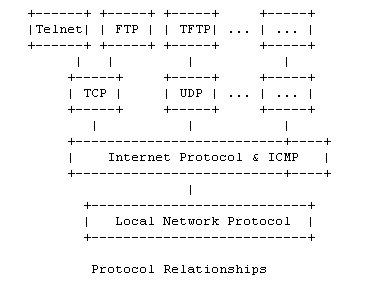
\includegraphics[width=0.8\textwidth]{\resdir/protocol_relationship.jpg}

\end{frame}
% ----------------------------------------------------------------------


% ----------------------------------------------------------------------
\begin{frame}{Protocoles de Communication Applicatives Sp�cifiques}

	\centering
	
	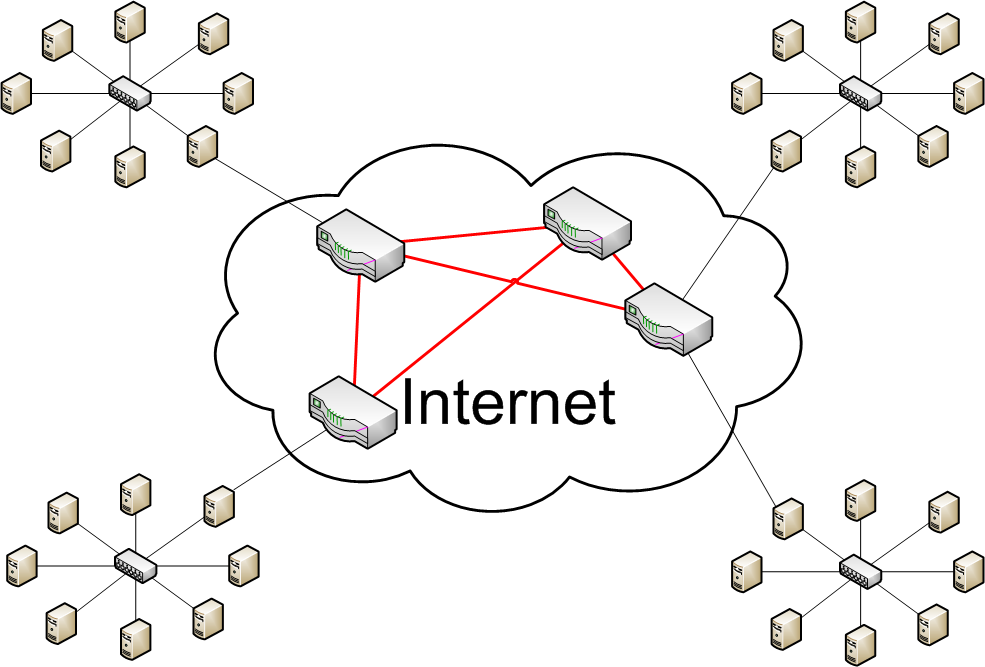
\includegraphics[height=0.4\textheight]{\resdir/internet}
	
	\begin{block}<+-> {Ajoute du service}
		\begin{itemize}
			\item D�di� � une application particuli�re
			\item Tr�s nombreux
				\begin{itemize}
				\item Telnet, FTP, Kad, AIM, Jabber
				\item Bas�s sur TCP/IP ou UDP/IP
				\end{itemize}
		\end{itemize}
	\end{block}
	
\end{frame}
% ----------------------------------------------------------------------

% ----------------------------------------------------------------------
\begin{frame}
	\begin{columns}
	
	\column{0.5\textwidth}
		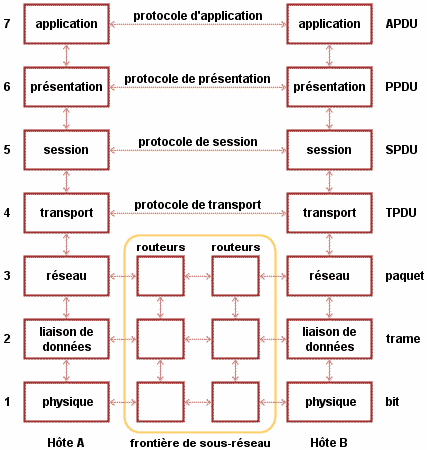
\includegraphics[height=0.8\textheight]{\resdir/osi}
	
	\column{0.5\textwidth}
		\begin{block}<+-> {Sp�cifiques}
			\begin{itemize}						
			\item Impl�mente la couche
				\begin{itemize}
				\item Application (7)
				\end{itemize}
			\item Empaquette l'information
				\begin{itemize}
				\item Dans un but pr�cis
				\end{itemize}
			\item Supporte les \textit{services}
			\end{itemize}
		\end{block}
		
	\end{columns}		
\end{frame}
% ----------------------------------------------------------------------

% ----------------------------------------------------------------------
\begin{frame}{Conclusion}
		
	\centering
	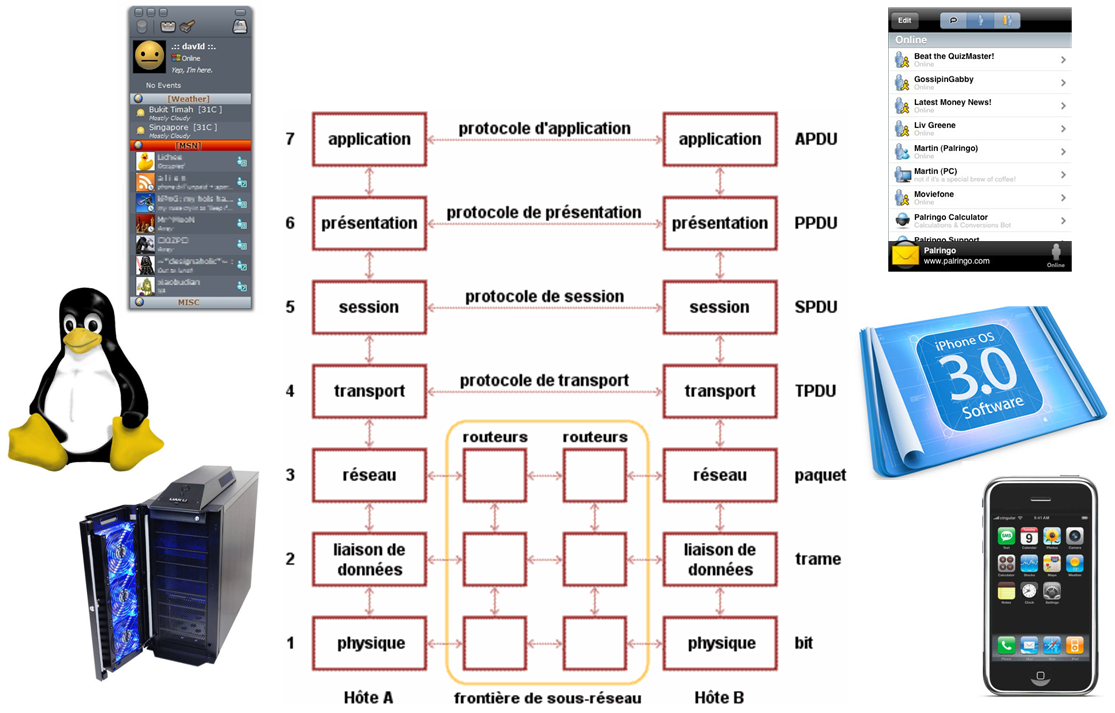
\includegraphics[height=0.8\textheight]{\resdir/osi++}

\end{frame}
% ----------------------------------------------------------------------

%
%\def\resdir{outils}

% ----------------------------------------------------------------------
\section{Outils}
% ----------------------------------------------------------------------

% ----------------------------------------------------------------------
\subsection{Outils}
% ----------------------------------------------------------------------

% ----------------------------------------------------------------------
\begin{frame}{Configuration IP (linux)}
	\centering
	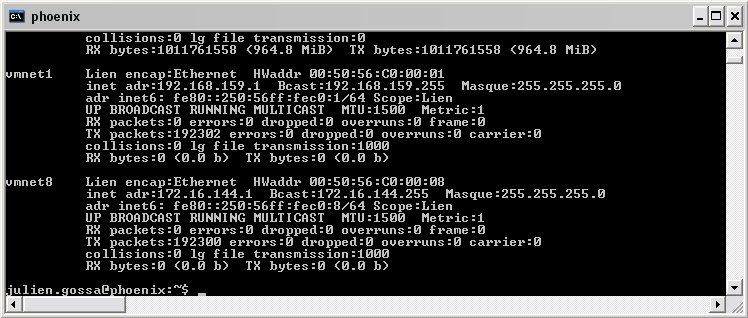
\includegraphics[width=\textwidth]{\resdir/ifconfig}
	
\end{frame}
% ----------------------------------------------------------------------

% ----------------------------------------------------------------------
\begin{frame}{Configuration IP (windows)}
	\centering
	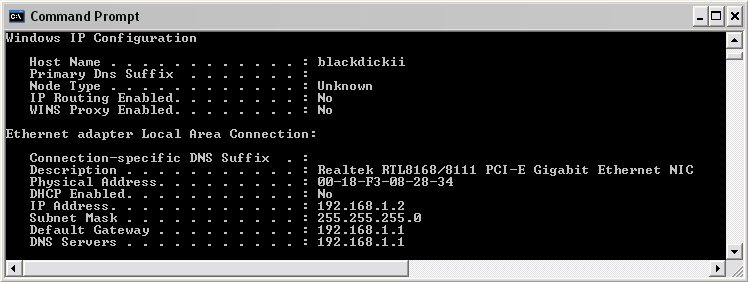
\includegraphics[width=\textwidth]{\resdir/ipconfig}
	
\end{frame}
% ----------------------------------------------------------------------

% ----------------------------------------------------------------------
\begin{frame}{Nom de machine $\Longleftrightarrow$ Adresse IP}
	\centering
	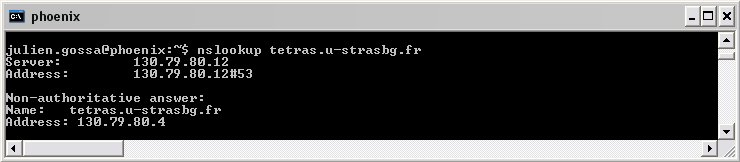
\includegraphics[width=\textwidth]{\resdir/nslookup}
	
\end{frame}
% ----------------------------------------------------------------------

% ----------------------------------------------------------------------
\begin{frame}{Ping}
	\centering
	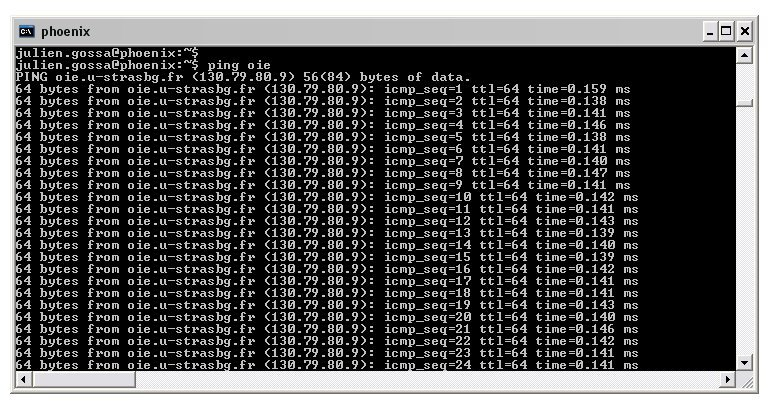
\includegraphics[width=\textwidth]{\resdir/ping}
	
\end{frame}
% ----------------------------------------------------------------------

% ----------------------------------------------------------------------
\begin{frame}{Route}
	\centering
	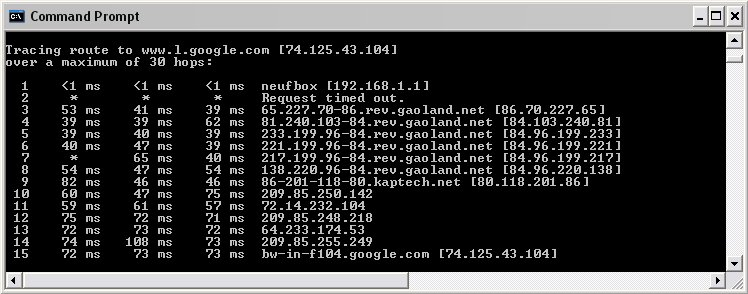
\includegraphics[width=\textwidth]{\resdir/tracert}
	
\end{frame}
% ----------------------------------------------------------------------

%
%
\def\resdir{4ethernet}

% ----------------------------------------------------------------------
\section{Ethernet}
% ----------------------------------------------------------------------

% ----------------------------------------------------------------------
\subsection{Adresse MAC}
% ----------------------------------------------------------------------

% ----------------------------------------------------------------------
\begin{frame}{Ethernet}
	\centering
	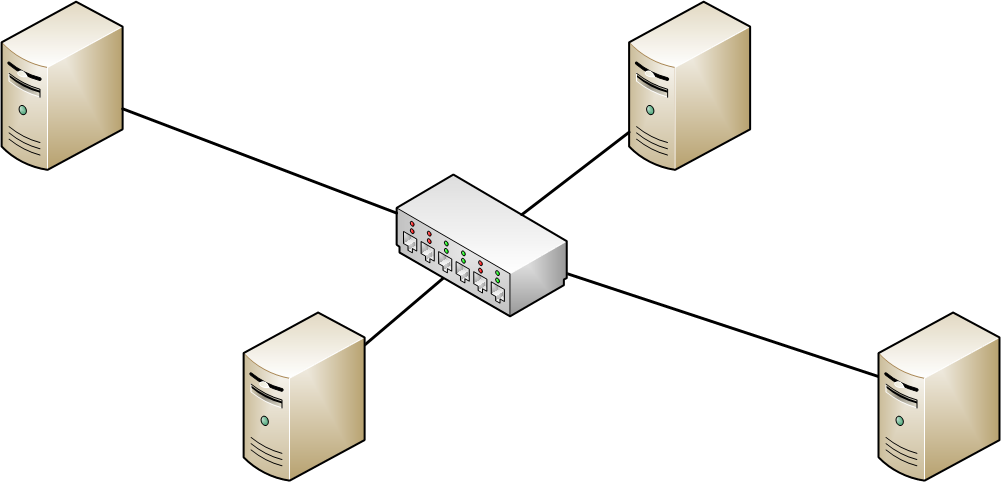
\includegraphics[height=0.4\textheight]{\resdir/etoile}
	
	\begin{block}<+-> {Ethernet - Topologie}
		\begin{itemize}
			\item En \'Etoile
			\item Autour d'un hub ou d'un switch
			\item Unique m�dium de communication
		\end{itemize}
	\end{block}
	
\end{frame}
% ----------------------------------------------------------------------

% ----------------------------------------------------------------------
\begin{frame}{\'Etoile autour d'un HUB}
	\centering
	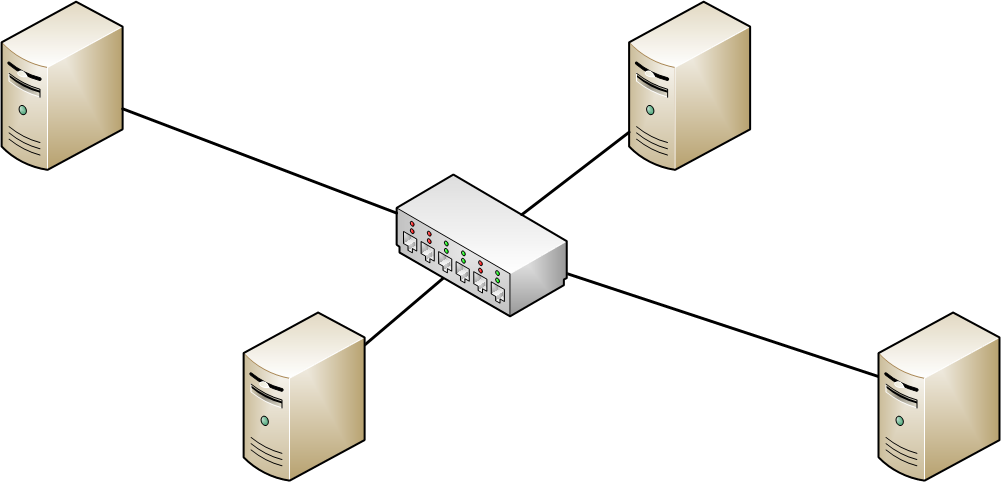
\includegraphics[height=0.6\textheight]{\resdir/etoile}
		
\end{frame}
% ----------------------------------------------------------------------
\begin{frame}{\'Etoile autour d'un HUB = BUS}
	\centering
	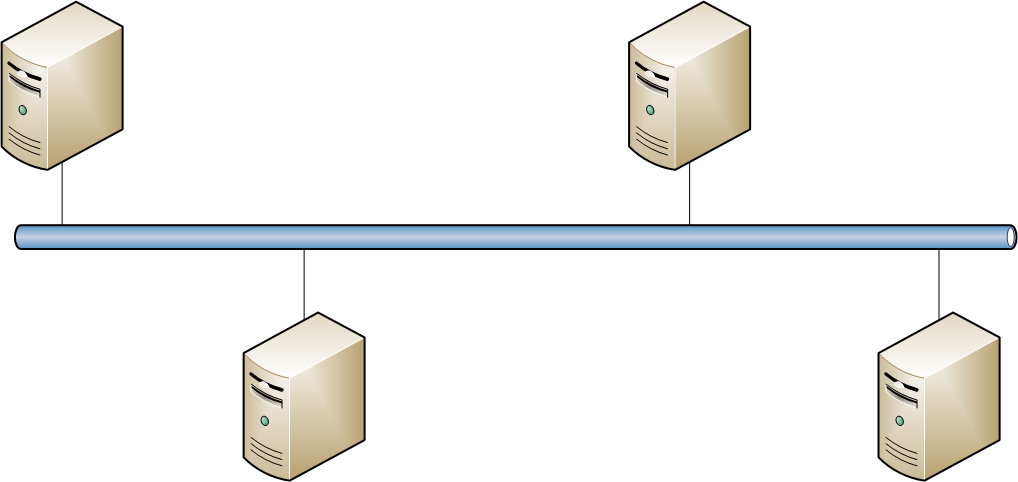
\includegraphics[height=0.6\textheight]{\resdir/bus1}
		
\end{frame}
% ----------------------------------------------------------------------
\begin{frame}{Communications montantes et descendante}
	\centering
	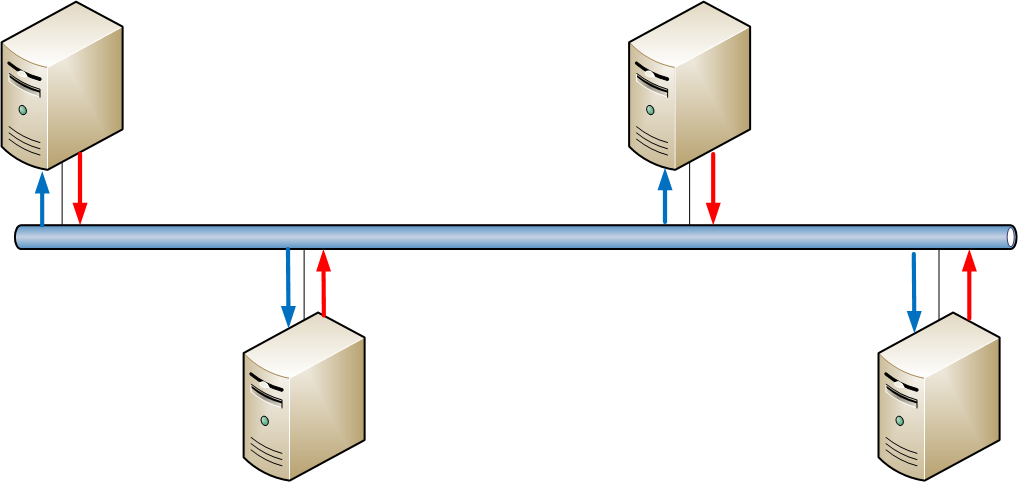
\includegraphics[height=0.6\textheight]{\resdir/bus2}
		
\end{frame}
% ----------------------------------------------------------------------
\begin{frame}{Adresse MAC (Media Access Control) pour filtrage}
	\centering
	\includegraphics[height=0.6\textheight]{\resdir/busmac}
		
\end{frame}
% ----------------------------------------------------------------------

% ----------------------------------------------------------------------
\subsection{Protocole Ethernet}
% ----------------------------------------------------------------------

% ----------------------------------------------------------------------
\begin{frame}{M�dium unique = unique \textit{parleur}}
	\centering
	\includegraphics[height=0.6\textheight]{\resdir/bus3}
		
\end{frame}
% ----------------------------------------------------------------------
\begin{frame}{Parole � tour de r�le}
	\centering
	\includegraphics[height=0.6\textheight]{\resdir/bus4}
		
\end{frame}
% ----------------------------------------------------------------------


% ----------------------------------------------------------------------
\begin{frame}{Ethernet - Protocole}
	
			\small
			\begin{enumerate}
			\item \textit{d�but de transmission :} Si le m�dia n'est pas utilis�, commencer la transmission, sinon aller � l'�tape 4
			\item \textit{transmission de l'information :} Si une collision est d�tect�e, continue � transmettre jusqu'� ce que le temps minimal pour un paquet soit d�pass� (pour s'assurer que tous les postes d�tectent la collision), puis aller � l'�tape 4
			\item \textit{fin d'une transmission r�ussie :} Indiquer la r�ussite au protocole du niveau sup�rieur et sortir du mode de transfert.
			\item \textit{c�ble occup� :} Attendre jusqu'� ce que le fil soit inutilis�.
			\item \textit{le c�ble est redevenu libre :} Attendre pendant un temps al�atoire, puis retourner � l'�tape 1, sauf si le nombre maximal d'essais de transmission a �t� d�pass�.
			\item \textit{nombre maximal d'essais de transmission d�pass� :} Annoncer l'�chec au protocole de niveau sup�rieur et sortir du mode de transmission.
			\end{enumerate}
		
\end{frame}
% ----------------------------------------------------------------------


% ----------------------------------------------------------------------
\subsection{Ethernet Commut�}
% ----------------------------------------------------------------------

% ----------------------------------------------------------------------
\begin{frame}{Ethernet Commut�}

	\centering
	\includegraphics[height=0.6\textheight]{\resdir/switchmac}
		
			\begin{itemize}
				\item Hub vs. switch
				\item Avantage ?
				\item Comment ca marche ?
			\end{itemize}
					
\end{frame}
% ----------------------------------------------------------------------

% ----------------------------------------------------------------------
\begin{frame}{Ethernet Commut�}

	\centering
	
	\includegraphics[height=0.6\textheight]{\resdir/switchmac1}
		
			\begin{itemize}
				\item Hub vs. switch
				\item Avantage ?
				\item Comment ca marche ?
			\end{itemize}
					
\end{frame}
% ----------------------------------------------------------------------

% ----------------------------------------------------------------------
\begin{frame}{Ethernet Commut�}

	\centering
	\includegraphics[height=0.6\textheight]{\resdir/switchmacport}
		
			\begin{tabular}{|c|c|}
				\hline
				MAC & Port \\
				\hline
				$5E:FF:56:A2:AF:15$ & $1$ \\ 
				$4E:7F:B6:AE:12:FD$ & $2$ \\
				$42:CC:12:2B:F7:51$ & $3$ \\
				$DF:14:DE:21:C7:D1$ & $4$ \\
				\hline
			\end{tabular}
					
\end{frame}
% ----------------------------------------------------------------------


%
\def\resdir{5internet}

% ----------------------------------------------------------------------
\section{Internet}
% ----------------------------------------------------------------------


% ----------------------------------------------------------------------
\begin{frame}{Inter-Network Protocols}

	\begin{block}<+-> {Deux niveaux g�n�riques basiques}
	\begin{itemize}
		\item R�seau Local : Ethernet
		\item R�seau Global : Internet
		\begin{itemize}
			\item Internet Protocol (IP) d�crit dans la RFC 791				
			\item \url{http://tools.ietf.org/html/rfc791}
			\end{itemize}
		\end{itemize}					
		\end{block}
		
		\centering
		\includegraphics[width=\textwidth]{\resdir/gateways_protocol.jpg}

\end{frame}
% ----------------------------------------------------------------------

% ----------------------------------------------------------------------
\begin{frame}

	\centering
	
	\includegraphics[height=0.95\textheight]{\resdir/carte-internet}
	
\end{frame}
% ----------------------------------------------------------------------
%
%% ----------------------------------------------------------------------
%\begin{frame}
%	\begin{columns}
%	
%	\column{0.5\textwidth}
%		\includegraphics[height=0.8\textheight]{\resdir/osi_com}
%	
%	\column{0.5\textwidth}
%		\begin{block}<+-> {IP}
%			\begin{itemize}
%			
%			\item Couche Application
%				\begin{itemize}
%					\item applications standard du r�seau 
%					\item Telnet, SMTP, FTP\ldots
%				
%			\item Couche Transport
%				\begin{itemize}
%					\item Acheminement et �tat transmission
%				\end{itemize}
%							
%			\item Couche Internet 
%				\begin{itemize}
%					\item paquet de donn�es (datagramme)
%				\end{itemize}
%							
%			\item Couche Acc�s r�seau
%				\begin{itemize}
%					\item Forme des donn�es
%				\end{itemize}
%			
%				
%				\end{itemize}
%			\end{itemize}
%		\end{block}
%		
%	\end{columns}		
%\end{frame}
%% ----------------------------------------------------------------------


% ----------------------------------------------------------------------
\begin{frame}
	\begin{columns}
	
	\column{0.5\textwidth}
		\hspace*{-0.5cm}
		\includegraphics[height=0.8\textheight]{\resdir/osi}
	
	\column{0.5\textwidth}
		\begin{block}<+-> {IP : Internet Protocol}
			\begin{itemize}
			\item Protocole R�seau de R�seaux
			\item Rout�
				\item Impl�mentation de la couche
				\begin{itemize}
					\item R�seau
				\end{itemize}
				\item Inter - Net(work)
				\item Bas� sur l'adresse IP
				\begin{itemize}
					\item IPv4 ou IPv6
				\end{itemize}
				\item \'Echange de \textit{Paquets}
			\end{itemize}
		\end{block}
		
	\end{columns}		
\end{frame}
% ----------------------------------------------------------------------



% ----------------------------------------------------------------------
\begin{frame}{IP : Internet Protocole}

			\begin{itemize}
%				\item Suite de protocoles 
%				\item Transmission Control Protocol/Internet Protocol
				\item Ensemble des r�gles de communication sur Internet
				\item Internet = r�seau des r�seaux
				\item IP communication des r�seaux entre eux
			\end{itemize}

		\begin{alertblock}<2-> {Services}
			\begin{itemize}
				\item Fractionnement des messages en paquets
    		\item Utilisation du syst�me d'adressage IP
    		\item Acheminement des donn�es sur le r�seau (routage)
%    		\item Contr�le des erreurs de transmission de donn�es
			\end{itemize}		
		\end{alertblock}
					
\end{frame}
% ----------------------------------------------------------------------

% ----------------------------------------------------------------------
\begin{frame}{Internet et IP}

	\centering
	
	\includegraphics[height=0.85\textheight]{\resdir/bout-en-bout}
	
\end{frame}
% ----------------------------------------------------------------------

\section{Adresses IPv4}

% ----------------------------------------------------------------------
\begin{frame}{Adresses IPv4}
		
		
			\begin{itemize}
				\item Identifie une interface
				\item Adresses IP g�r�es et vendues par l'ICANN 
					\begin{itemize}
					\item Internet Corporation for Assigned Names and Numbers, 
					\item rempla�ant l'IANA, Internet Assigned Numbers Agency, depuis 1998
					\end{itemize}	
			\end{itemize}

				\begin{block}<2->{Suite de 4 octets / 32 bits s�par�s par des ``.''}
					\begin{tt}
					\begin{tabular}{cccccccc}
					91 & . & 198 & . & 174 & . & 2 \\
					01011011 & . & 11000110 & . & 10101110 & . & 00000010 \\
					\end{tabular}
					\end{tt}
				\end{block}

		
\end{frame}
% ----------------------------------------------------------------------


% ----------------------------------------------------------------------
\begin{frame}{Adresses IPv4 : Internet}

	\centering
	
	\includegraphics[height=0.85\textheight]{\resdir/ipnet}
	
\end{frame}
% ----------------------------------------------------------------------

% ----------------------------------------------------------------------
\begin{frame}

	\centering
	
	\includegraphics[height=0.95\textheight]{\resdir/carte-internet}
	
\end{frame}
% ----------------------------------------------------------------------

% ----------------------------------------------------------------------
\begin{frame}{Adresses IPv4 : Deux parties }

	\begin{itemize}
	\item \textbf{r�seau} (\textit{netid}) : routage sur internet
	\item \textbf{h�te} (\textit{hostid}) : routage � l'int�rieur du r�seau
	\end{itemize}
	
	\vspace*{0.3cm}
	\centering
	
	\includegraphics[height=0.70\textheight]{\resdir/ipnet}
							
\end{frame}
% ----------------------------------------------------------------------

\section{R�seau}

% ----------------------------------------------------------------------
\begin{frame}{Adresses IPv4 : Classe}

			Organisation par classes
			\begin{itemize}
			\item D�fini la longueur des parties r�seau et h�te
			\item On achete une \textit{plage} d'adresse d�finie par la partie h�te
			\end{itemize}

		\begin{block}<2-> {Classes}
			\begin{description}
			\item [Classe A] : 1 octet r�seau, commence par \hfill \texttt{0\ \ \ \ldots}
			\item [Classe B] : 2 octets r�seau, commence par \hfill \texttt{10\ \ \ldots}
			\item [Classe C] : 3 octets r�seau, commence par \hfill \texttt{110\ \ldots}
			\item [Classe D] : multicast, commence par \hfill \texttt{1110\ldots}
			\item [Classe E] : exp�rimental, le reste
			\end{description}
		\end{block}		
	
\end{frame}
% ----------------------------------------------------------------------


% ----------------------------------------------------------------------
\begin{frame}%{Adresses IPv4 : Classe et plages d'adresse }

		\footnotesize
		\begin{tt}
		\begin{tabular}{|l|c|c|}
							\hline
		 					& 00000000.00000000.00000000.00000000 &	\ \ 0.\ \ 0.\ \ 0.\ \ 0 	 \\
		 					& . & . \\ & . & . \\ & . & . \\ & . & . \\ & . & . \\ 
		 					Classe A & . & . \\ & . & . \\ & . & . \\ & . & . \\ & . & .  \\ 
		 					& 01111111.11111111.11111111.11111111	& 127.255.255.255 \\
		 					\hline
		 					& 10000000.00000000.00000000.00000000 &	128.\ \ 0.\ \ 0.\ \ 0 	 \\
		 					& . & . \\ & . & . \\ Classe B & . & .  \\ & . & . \\ & . & . \\
		 					& 10111111.11111111.11111111.11111111 &	191.255.255.255 	 \\
		 					\hline
		 					& 11000000.00000000.00000000.00000000 &	192.\ \ 0.\ \ 0.\ \ 0 	 \\
		 					Classe C & . & . \\ & . & . \\
		 					& 11011111.11111111.11111111.11111111 &	223.255.255.255 	 \\
		 					\hline
Classe D\&E	& 11100000.00000000.00000000.00000000 &	224.\ \ 0.\ \ 0.\ \ 0 	 \\
		 					& 11111111.11111111.11111111.11111111	& 255.255.255.255 \\
							\hline
		\end{tabular}
		\normalsize
		\end{tt}
		
		
\end{frame}
% ----------------------------------------------------------------------


% ----------------------------------------------------------------------
\begin{frame}{Adresses IPv4 : Classes }

	\centering
	
	\includegraphics[height=0.85\textheight]{\resdir/ipnet}
							
\end{frame}
% ----------------------------------------------------------------------


%TODO : metter classe B et C
% ----------------------------------------------------------------------
\begin{frame}{Adresses IPv4 : Masque}

		\begin{block}<+-> {Masque par d�faut}
			\begin{itemize}
			\item 32 bits, certains � \texttt{1} suivis de bits � \texttt{0}
			\item D�fini par le nombre de bits � \texttt{1}, selon la classe	
			\item Permet de retrouver :
				\begin{itemize}
				\item La partie r�seau  par un ET
				\item La partie h�te  par un ET avec son compl�ment bit � bit
				\end{itemize}
			\end{itemize}		
		\end{block}
		
		\vspace*{0.3cm}

		\only<1>{
		Classe A : Masque de 8 bits (1 octet)
		
		\vspace*{0.3cm}
		\footnotesize
		\hspace*{-0.5cm}
		\begin{tabular}{lcl}
		Adresse IPv4 								& \texttt{01011011.11000110.10101110.00000010}
																&	\texttt{\ 91.198.174.\ \ 2} 	 \\
		Masque par d�faut 					& \texttt{\textcolor{red}{11111111}.\textcolor{blue}{00000000.00000000.00000000}}
																&	\texttt{\textcolor{red}{255}.\textcolor{blue}{\ \ 0.\ \ 0.\ \ 0}} \\
		\hline\\
		R�seau 											& \texttt{\textcolor{red}{01011011}.00000000.00000000.00000000}
																&	\texttt{\textcolor{red}{\ 91}.\ \ 0.\ \ 0.\ \ 0} \\
		H�te 												&	\texttt{00000000.\textcolor{blue}{11000110.10101110.00000010}}
							 									&	\texttt{\ \ 0.\textcolor{blue}{198.174.\ \ 2}} \\
		\\\hline\\
		Adresse IPv4 								& \texttt{\textcolor{red}{01011011}.\textcolor{blue}{11000110.10101110.00000010}}
																&	\texttt{\textcolor{red}{\ 91}.\textcolor{blue}{198.174.\ \ 2}} 	 \\
		\end{tabular}
		\normalsize
		}
		
		\only<2>{
		Classe B : Masque de 16 bits (2 octets)
		
		\vspace*{0.3cm}
		\footnotesize
		\hspace*{-0.5cm}
		\begin{tabular}{lcl}
		Adresse IPv4 								& \texttt{10000010.11000110.10101110.00000010}
																&	\texttt{130.198.174.\ \ 2} 	 \\
		Masque par d�faut 					& \texttt{\textcolor{red}{11111111.11111111}.\textcolor{blue}{00000000.00000000}}
																&	\texttt{\textcolor{red}{255.255}.\textcolor{blue}{\ \ 0.\ \ 0}} \\
		\hline\\
		R�seau 											& \texttt{\textcolor{red}{10000010.11000110}.00000000.00000000}
																&	\texttt{\textcolor{red}{130.198}.\ \ 0.\ \ 0} \\
		H�te 												&	\texttt{00000000.00000000.\textcolor{blue}{10101110.00000010}}
							 									&	\texttt{\ \ 0.\ \ 0.\textcolor{blue}{174.\ \ 2}} \\
		\\\hline\\
		Adresse IPv4 								& \texttt{\textcolor{red}{10000010.11000110}.\textcolor{blue}{10101110.00000010}}
																&	\texttt{\textcolor{red}{130.198}.\textcolor{blue}{174.\ \ 2}} 	 \\
		\end{tabular}
		\normalsize
		}
		
		\only<3>{
		Classe C : Masque de 24 bits (3 octets)
		
		\vspace*{0.3cm}
		\footnotesize
		\hspace*{-0.5cm}
		\begin{tabular}{lcl}
		Adresse IPv4 								& \texttt{11001000.11000110.10101110.00000010}
																&	\texttt{200.198.174.\ \ 2} 	 \\
		Masque par d�faut 					& \texttt{\textcolor{red}{11111111.11111111.11111111}.\textcolor{blue}{00000000}}
																&	\texttt{\textcolor{red}{255.255.255}.\textcolor{blue}{\ \ 0}} \\
		\hline\\
		R�seau 											& \texttt{\textcolor{red}{11001000.11000110.10101110}.00000000}
																&	\texttt{\textcolor{red}{200.198.174}.\ \ 0} \\
		H�te 												&	\texttt{00000000.00000000.00000000.\textcolor{blue}{00000010}}
							 									&	\texttt{\ \ 0.\ \ 0.\ \ 0.\textcolor{blue}{\ \ 2}} \\
		\\\hline\\
		Adresse IPv4 								& \texttt{\textcolor{red}{11001000.11000110.10101110}.\textcolor{blue}{00000010}}
																&	\texttt{\textcolor{red}{130.198.174}.\textcolor{blue}{\ \ 2}} 	 \\
		\end{tabular}
		\normalsize
		}	
		
		\only<4>{
		Classe D\&E : Masque de 8 bits (4 octets)
		
		\vspace*{0.3cm}
		\footnotesize
		\hspace*{-0.5cm}
		\begin{tabular}{lcl}
		Adresse IPv4 								& \texttt{11100001.11000110.10101110.00000010}
																&	\texttt{225.198.174.\ \ 2} 	 \\
		Masque par d�faut 					& \texttt{\textcolor{red}{11111111.11111111.11111111.11111111}}
																&	\texttt{\textcolor{red}{255.255.255.255}} \\
		\hline\\
		R�seau 											& \texttt{\textcolor{red}{11100001.11000110.10101110.00000010}}
																&	\texttt{\textcolor{red}{225198.174.\ \ 2}} \\
		H�te 												&	\texttt{00000000.00000000.00000000.00000000}
							 									&	\texttt{\ \ 0.\ \ 0.\ \ 0.\ \ 0} \\
		\\\hline\\
		Adresse IPv4 								& \texttt{\textcolor{red}{11100001.11000110.10101110.00000010}}
																&	\texttt{\textcolor{red}{225.198.174.\ \ 2}} 	 \\
		\end{tabular}
		\normalsize
		}
		
\end{frame}
% ----------------------------------------------------------------------



\section{Sous-r�seau}


% ----------------------------------------------------------------------
\begin{frame}{Sous-r�seau}

		\begin{itemize}
		\item<+-> R�seau potentiellement grand
			\begin{itemize}
			\item Classe A : 16 millions d'h�tes par r�seau
			\end{itemize}
		\item<+-> Impossible en r�seau local
		\item<+-> Besoin de pouvoir d�couper un r�seau
		\end{itemize}
		
		\begin{block}<+->{Notion de sous-r�seau}
			\begin{itemize}
			\item Permet de d�couper un r�seau donn�
			\item En plusieurs sous-r�seaux
			\item Permet le routage � l'int�rieur d'un r�seau
			\end{itemize}
		\end{block}
			
\end{frame}
% ----------------------------------------------------------------------

% ----------------------------------------------------------------------
\begin{frame}{Adresses IPv4 : R�seau }

	\centering
	
	\includegraphics[height=0.85\textheight]{\resdir/reseau}
							
\end{frame}
% ----------------------------------------------------------------------



% ----------------------------------------------------------------------
\begin{frame}{Adresses IPv4 : Sous-R�seaux}

	\centering
	
	\includegraphics[height=0.85\textheight]{\resdir/sousreseau}
							
\end{frame}
% ----------------------------------------------------------------------



% ----------------------------------------------------------------------
\begin{frame}{Sous-r�seau : Masque}

		D�fini par le nombre de bits � 1
				\begin{itemize}
				\item<+-> Ex : \texttt{91.198.174.2\textbf{/24}} \hfill Masque = \texttt{255.255.255.0}
				\end{itemize}			
				
		\begin{block}<+->{Permet de retrouver :}
			\begin{itemize}
			\item La partie r�seau �tendu 
			\item La partie sous-r�seau
			\item La partie h�te dans le sous-r�seau
			\end{itemize}
		\end{block}

		\uncover<+->{
		\footnotesize
		\vspace{0.3cm}
		\hspace*{-0.5cm}
		\begin{tabular}{lcl}
		Adresse IPv4 								& \texttt{\textcolor{red}{01010010}.\textcolor{magenta}{00001010.00011110}.\textcolor{blue}{00000010}}
																&	\texttt{\textcolor{red}{\ 82}.\textcolor{magenta}{\ 10.\ 30}.\textcolor{blue}{2}/24}	 \\
		Masque par d�faut 					& \texttt{\textcolor{red}{11111111}.\textcolor{magenta}{00000000.00000000}.\textcolor{blue}{00000000}}
																&	\texttt{\textcolor{red}{255}.\textcolor{magenta}{\ \ 0.\ \ 0}.\textcolor{blue}{0}} \\
		Masque de S-R								& \texttt{\textcolor{red}{11111111}.\textcolor{magenta}{11111111.11111111}.\textcolor{blue}{00000000}}
																&	\texttt{\textcolor{red}{255}.\textcolor{magenta}{255.255}.\textcolor{blue}{0}} \\													\\
		R�seau											& \texttt{\textcolor{red}{01010010}.\textcolor{magenta}{00000000.00000000}.\textcolor{blue}{00000000}}
																&	\texttt{\textcolor{red}{\ 82}.\textcolor{magenta}{\ \ 0.\ \ 0}.\textcolor{blue}{0}} \\		
		\\
		R�seau �tendu								& \texttt{\textcolor{red}{01010010}.\textcolor{magenta}{00001010.00011110}.\textcolor{blue}{00000000}}
																&	\texttt{\textcolor{red}{\ 82}.\textcolor{magenta}{\ 10.\ 30}.\textcolor{blue}{0}} \\
		\\
		Sous-r�seau									&	\texttt{\textcolor{red}{00000000}.\textcolor{magenta}{00001010.00011110}.\textcolor{blue}{00000000}}
							 									&	\texttt{\textcolor{red}{\ \ 0}.\textcolor{magenta}{\ 10.\ 30}.\textcolor{blue}{2}} \\
		\\ H�te dans S-R						&	\texttt{\textcolor{red}{00000000}.\textcolor{magenta}{00000000.00000000}.\textcolor{blue}{00000010}}
							 									&	\texttt{\textcolor{red}{\ \ 0}.\textcolor{magenta}{\ \ 0.\ \ 0}.\textcolor{blue}{2}} \\							 									
		\end{tabular}
		\normalsize
		}

\end{frame}
% ----------------------------------------------------------------------



% ----------------------------------------------------------------------
\begin{frame}{Sous-R�seaux : Interconnexion}

	\centering
	
	\includegraphics[height=0.85\textheight]{\resdir/sousreseau}
							
\end{frame}
% ----------------------------------------------------------------------

\section{Adresses particuli�res}

% ----------------------------------------------------------------------
\begin{frame}{Adresses particuli�res}

		\begin{block}<+-> {Par masque (ex classe A sans sous-r�seau)}
			\begin{itemize}
			\item \texttt{\ \ X.\textcolor{blue}{\ \ 0.\ \ 0.\ \ 0}} : adresse r�seau
			\item \texttt{\ \ X.\textcolor{blue}{255.255.255}}  : adresse (\textit{broadcast})
			\item \texttt{\textcolor{red}{\ \ 0}.\ \ X.\ \ X.\ \ X} : adresse h�te dans le sous-r�seau courant
			\item \texttt{\textcolor{red}{255}.\ \ X.\ \ X.\ \ X} : adresse (\textit{multicast})
			\item \texttt{\textcolor{red}{255}.\textcolor{blue}{255.255.255}} : adresse (\textit{broadcast universel}) 			
			\end{itemize}		
		\end{block}
		
		\begin{block}<+-> {Adresses priv�es}
			\begin{itemize}
			\item L'adresse de classe A 10.0.0.0 
			\item Les adresses r�seau de classe B 172.16.0.0 � 172.31.0.0 
			\item Les adresses r�seau de classe C 192.168.0.0 � 192.168.255.0 
			\end{itemize}
		\end{block}

		\begin{block}<+-> {Boucle locale}
			\begin{itemize}
			\item 127.0.0.1 = \textit{localhost}
			\end{itemize}		
		\end{block}
		
\end{frame}

% ----------------------------------------------------------------------



\def\resdir{5internet}

% ----------------------------------------------------------------------
\section{Plan d'adressage}
% ----------------------------------------------------------------------

% ----------------------------------------------------------------------
\subsection{Construction du plan d'adressage}
% ----------------------------------------------------------------------

% ----------------------------------------------------------------------
\begin{frame}
	\begin{columns}
	
	\column{0.5\textwidth}
		\hspace*{-0.5cm}
		\includegraphics[height=0.8\textheight]{\resdir/osi}
	
	\column{0.5\textwidth}
		\begin{block}<+-> {IP : Internet Protocol}
			\begin{itemize}
			\item Protocole R�seau de R�seaux
			\item Rout�
				\item Impl�mentation de la couche
				\begin{itemize}
					\item R�seau
				\end{itemize}
				\item Inter - Net(work)
				\item Bas� sur l'adresse IP
				\begin{itemize}
					\item IPv4 ou IPv6
				\end{itemize}
				\item \'Echange de \textit{Paquets}
			\end{itemize}
		\end{block}
		
	\end{columns}		
\end{frame}
% ----------------------------------------------------------------------


% ----------------------------------------------------------------------
\begin{frame}

	\centering
	
	\includegraphics[height=0.95\textheight]{\resdir/reseau-vierge}
	
\end{frame}
% ----------------------------------------------------------------------


% ----------------------------------------------------------------------
\begin{frame}{Plan d'adressage}

	\centering
	\includegraphics[height=0.4\textheight]{\resdir/reseau-vierge}

	\begin{itemize}
		\item<+-> On dispose de l'adresse \texttt{192.1.1.0/24}
		\item<+-> Plage : \texttt{192.1.1.0 - 192.1.1.255} (classe C)
		\item<+-> Comment attribuer les adresses aux machines ?
	\end{itemize}
	
	\only<1-7>{
	\begin{block}<+->{Objectifs}
		\begin{itemize}
			\item<+-> Partitionner le r�seau
			\item<+-> Optimiser l'utilisation de la plage
			\item<+-> Permettre le routage interne des paquets
		\end{itemize}
	\end{block}
	}\only<8->{
	\begin{block}{M�thode}
		\begin{itemize}
			\item<9-> Attribuer des plages aux sous-r�seaux
			\item<10-> Au plus juste, mais non satur�es
			\item<11-> Par ordre d�croissant du nombre d'adresses
		\end{itemize}
	\end{block}
	}

\end{frame}
% ----------------------------------------------------------------------

% ----------------------------------------------------------------------
\begin{frame}{Plan d'adressage : M�thode}

	\centering
	
	\includegraphics[height=0.4\textheight]{\resdir/reseau-vierge}
	
	\begin{block}<1-3>{Attribuer des plages aux sous-r�seaux}
 		Plage \texttt{192.1.1.X/M} : Trouver \texttt{M}, puis \texttt{X}
	\end{block}
	
	\begin{block}<2-3>{Au plus juste, mais non satur�es}
		\texttt{M} doit �tre le plus petit possible, tout en laissant des adresses libres
	\end{block}
	
	\begin{block}<3-3>{Par ordre d�croissant du nombre de machines}
		Contrainte technique
	\end{block}	
		
\end{frame}
% ----------------------------------------------------------------------


% ----------------------------------------------------------------------
\begin{frame}{Plan d'adressage : M�thode - Trouver \texttt{M}}

\uncover<+->{Plage \texttt{192.1.1.X/M} : $M=32-nb\ bits\ necessaires\ pour\ les\ hotes$}

 	\begin{itemize}
 	\item<+-> \textbf{\texttt{M}=30} : $32-M=2\ bits\ hote \Rightarrow 4\ adresses \Rightarrow 2\ adresses\ utiles$
\uncover<+->{
 		\hspace*{-1.5cm}\footnotesize	\begin{tt}
		\begin{tabular}{lcl}
Masque de S-R &
\textcolor{red}{11000000.11111111.11111111}.\textcolor{magenta}{111111}\textcolor{blue}{00} & 255.255.255.252 \\
Adresse IPv4 & 
\textcolor{red}{11000000.00000001.00000001}.\textcolor{magenta}{xxxxxx}\textcolor{blue}{xx} & 192.\ \ 1.\ \ 1.XXX \\
		\end{tabular}
		\end{tt} \normalsize	
}

\uncover<+->{ Plage d'adresse :
 		\hspace*{-1.5cm}\footnotesize	\begin{tt}
		\begin{tabular}{lcl}
		\hline
@ R�seau
& \textcolor{red}{11000000.00000001.00000001}.\textcolor{magenta}{xxxxxx}\textcolor{blue}{00} & 192.\ \ 1.\ \ 1.0 \\
\phantom{Masque de S-R}
& \textcolor{red}{11000000.00000001.00000001}.\textcolor{magenta}{xxxxxx}\textcolor{blue}{01} & 192.\ \ 1.\ \ 1.1 \\
& \textcolor{red}{11000000.00000001.00000001}.\textcolor{magenta}{xxxxxx}\textcolor{blue}{10} & 192.\ \ 1.\ \ 1.2 \\
@ Broadcast
& \textcolor{red}{11000000.00000001.00000001}.\textcolor{magenta}{xxxxxx}\textcolor{blue}{11} & 192.\ \ 1.\ \ 1.3 \\
\hline
		\end{tabular}
		\end{tt} \normalsize	
}
 	\item<+-> \textbf{\texttt{M}=29} : $32-M=3\ bits\ hote \Rightarrow 8\ adresses \Rightarrow 6\ adresses\ utiles$
 	
 		\hspace*{-1.5cm}\footnotesize	\begin{tt}
		\begin{tabular}{lcl}
Masque de S-R &
\textcolor{red}{11000000.11111111.11111111}.\textcolor{magenta}{11111}\textcolor{blue}{000} & 255.255.255.248 \\
Adresse IPv4 & 
\textcolor{red}{11000000.00000001.00000001}.\textcolor{magenta}{xxxxx}\textcolor{blue}{xxx} & 192.\ \ 1.\ \ 1.XXX \\
		\end{tabular}
		\end{tt} \normalsize		
		
	\item<+-> \ldots	
		
 	\item<+-> \textbf{\texttt{M}=25} : $32-M=7\ bits\ hote \Rightarrow 128\ adresses \Rightarrow 126\ adresses\ utiles$
 	 	
 		\hspace*{-1.5cm}\footnotesize	\begin{tt}
		\begin{tabular}{lcl}
Masque de S-R &
\textcolor{red}{11000000.11111111.11111111}.\textcolor{magenta}{1}\textcolor{blue}{0000000} & 255.255.255.128 \\
Adresse IPv4 & 
\textcolor{red}{11000000.00000001.00000001}.\textcolor{magenta}{x}\textcolor{blue}{xxxxxxx} & 192.\ \ 1.\ \ 1.XXX \\
		\end{tabular}
		\end{tt} \normalsize			
		 	
 	\end{itemize}
		
\end{frame}
% ----------------------------------------------------------------------

% ----------------------------------------------------------------------
\begin{frame}{Plan d'adressage : M�thode - Trouver \texttt{X}}

\begin{exampleblock}{Plage \texttt{192.1.1.X/M}}

\begin{itemize}
\item \texttt{X} = adresse du sous-r�seau
\item Premi�re adresse disponible suivante
\end{itemize}

\end{exampleblock}

\end{frame}
% ----------------------------------------------------------------------

% ----------------------------------------------------------------------
\begin{frame}{Plan d'adressage : Application}

	\centering
	
	\includegraphics[height=0.5\textheight]{\resdir/reseau-vierge}
		
	\begin{exampleblock}<+->{Par ordre d�croissant du nombre de machines}
		\begin{itemize}
		\item Sous-r�seau A : 80 machines
		\item Sous-r�seau B : 15 machines
		\item Sous-r�seau C : 6 machines
		\end{itemize}
	\end{exampleblock}
	
\end{frame}
% ----------------------------------------------------------------------


% ----------------------------------------------------------------------
\begin{frame}{Plan d'adressage : Application}
		
	\begin{exampleblock}<+->{Au plus juste, non satur�}
		\begin{itemize}
		\item<+-> Sous-r�seau A
			\begin{itemize}
			\item<+-> $2^6(64) \leq \mathbf{80+2} < 2^7(128) \Rightarrow 7 bits \Rightarrow M=32-7$
			\item<+-> $M=25$
			\item<+-> \texttt{11111111.11111111.11111111.10000000 \\ \ \ \ \ \ 255.\ \ \ \ \ 255.\ \ \ \ \ 255.\ \ \ \ \ 128}
			\end{itemize}
			
		\item<+-> Sous-r�seau B (ne pas oublier les 2 adresses r�serv�es)
			\begin{itemize}
			\item $2^4(16) \leq \mathbf{15+2} < 2^5(32) \Rightarrow 5 bits \Rightarrow M=32-5=27$
			\item $M=27$
			\item \texttt{11111111.11111111.11111111.11100000  \\ \ \ \ \ \ 255.\ \ \ \ \ 255.\ \ \ \ \ 255.\ \ \ \ \ 224}
			\end{itemize}
		
		\item<+-> Sous-r�seau C (non satur�)
			\begin{itemize}
			\item $2^3(8) \leq \mathbf{6+2} < 2^4(16) \Rightarrow 4 bits \Rightarrow M=32-4=28$
			\item $M=28$
			\item \texttt{11111111.11111111.11111111.11110000  \\ \ \ \ \ \ 255.\ \ \ \ \ 255.\ \ \ \ \ 255.\ \ \ \ \ 240}
			\end{itemize}
					
		\end{itemize}
	\end{exampleblock}
	
\end{frame}
% ----------------------------------------------------------------------


% ----------------------------------------------------------------------
\begin{frame}{Plan d'adressage : Application}

		
		\hspace*{-1cm} \footnotesize	\begin{tt}
		\begin{tabular}{|ll|ll|}

\hline

\textcolor{red}{11000000.00000001.00000001}.00000000 & 192.1.1.0  & \phantom{@R} & \phantom{192.1.1.128/27} \\
\ldots & & & \\
\ldots & & & \\
\ldots & & & \\



\ldots & & & \\
\ldots & & & \\
\ldots & & & \\
\ldots & & & \\



\ldots & & & \\
\ldots & & & \\
\ldots & & & \\
\ldots & & & \\


\ldots & & & \\
\ldots & & & \\
\textcolor{red}{11000000.00000001.00000001}.11111111 & 255.1.1.255 & & \\

\hline

		\end{tabular}
		\end{tt} 


\end{frame}
% ----------------------------------------------------------------------


% ----------------------------------------------------------------------
\begin{frame}{Plan d'adressage : Application}

		
		\hspace*{-1cm} \footnotesize	\begin{tt}
		\begin{tabular}{|ll|ll|}

\hline


\textcolor{red}{11000000.00000001.00000001}.\textcolor{magenta}{0}\textcolor{blue}{0000000} & 192.1.1.0\ \  & @R & \\
\textcolor{red}{11000000.00000001.00000001}.\textcolor{magenta}{0}\textcolor{blue}{0000000} & 192.1.1.1\ \  & @P & Sous-r�seau A\\
\ldots & & @H &  \scriptsize 192.1.1.0/25 \\
\textcolor{red}{11000000.00000001.00000001}.\textcolor{magenta}{0}\textcolor{blue}{1111111} & 255.1.1.127 & @B & \\

\hline

\textcolor{red}{11000000.00000001.00000001}.10000000 & 192.1.1.128  & \phantom{@R} & \phantom{192.1.1.128/27} \\
\ldots & & & \\
\ldots & & & \\
\ldots & & & \\



\ldots & & & \\
\ldots & & & Reste \\
\ldots & & & \\
\ldots & & & \\


\ldots & & & \\
\ldots & & & \\
\textcolor{red}{11000000.00000001.00000001}.11111111 & 255.1.1.255 & & \\

\hline

		\end{tabular}
		\end{tt} 


\end{frame}
% ----------------------------------------------------------------------


% ----------------------------------------------------------------------
\begin{frame}{Plan d'adressage : Application}

		
		\hspace*{-1cm} \footnotesize	\begin{tt}
		\begin{tabular}{|ll|ll|}

\hline


\textcolor{red}{11000000.00000001.00000001}.\textcolor{magenta}{0}\textcolor{blue}{0000000} & 192.1.1.0\ \  & @R & \\
\textcolor{red}{11000000.00000001.00000001}.\textcolor{magenta}{0}\textcolor{blue}{0000000} & 192.1.1.1\ \  & @P & Sous-r�seau A\\
\ldots & & @H &  \scriptsize 192.1.1.0/25 \\
\textcolor{red}{11000000.00000001.00000001}.\textcolor{magenta}{0}\textcolor{blue}{1111111} & 255.1.1.127 & @B & \\

\hline

\textcolor{red}{11000000.00000001.00000001}.\textcolor{magenta}{100}\textcolor{blue}{00000} & 192.1.1.128 & @R & \\
\textcolor{red}{11000000.00000001.00000001}.\textcolor{magenta}{100}\textcolor{blue}{00001} & 192.1.1.129 & @P & Sous-r�seau B \\
\ldots & & @H & 192.1.1.128/27 \\
\textcolor{red}{11000000.00000001.00000001}.\textcolor{magenta}{100}\textcolor{blue}{11111} & 255.1.1.159 & @B & \\

\hline

\textcolor{red}{11000000.00000001.00000001}.10100000 & 192.1.1.160 &\phantom{@R}&\phantom{192.1.1.160/27}\\
\ldots & & & \\
\ldots & & & \\
\ldots & & &  Reste \\


\ldots & & & \\
\ldots & & & \\
\textcolor{red}{11000000.00000001.00000001}.11111111 & 255.1.1.255 & & \\

\hline

		\end{tabular}
		\end{tt} 


\end{frame}
% ----------------------------------------------------------------------


% ----------------------------------------------------------------------
\begin{frame}{Plan d'adressage : Application}

		
		\hspace*{-1cm} \footnotesize	\begin{tt}
		\begin{tabular}{|ll|ll|}

\hline

\textcolor{red}{11000000.00000001.00000001}.\textcolor{magenta}{0}\textcolor{blue}{0000000} & 192.1.1.0\ \  & @R & \\
\textcolor{red}{11000000.00000001.00000001}.\textcolor{magenta}{0}\textcolor{blue}{0000000} & 192.1.1.1\ \  & @P & Sous-r�seau A\\
\ldots & & @H &  \scriptsize 192.1.1.0/25 \\
\textcolor{red}{11000000.00000001.00000001}.\textcolor{magenta}{0}\textcolor{blue}{1111111} & 255.1.1.127 & @B & \\

\hline

\textcolor{red}{11000000.00000001.00000001}.\textcolor{magenta}{100}\textcolor{blue}{00000} & 192.1.1.128 & @R & \\
\textcolor{red}{11000000.00000001.00000001}.\textcolor{magenta}{100}\textcolor{blue}{00001} & 192.1.1.129 & @P & Sous-r�seau B \\
\ldots & & @H & 192.1.1.128/27 \\
\textcolor{red}{11000000.00000001.00000001}.\textcolor{magenta}{100}\textcolor{blue}{11111} & 255.1.1.159 & @B & \\

\hline

\textcolor{red}{11000000.00000001.00000001}.\textcolor{magenta}{1010}\textcolor{blue}{0000} & 192.1.1.160 & @R & \\
\textcolor{red}{11000000.00000001.00000001}.\textcolor{magenta}{1010}\textcolor{blue}{0001} & 192.1.1.161 & @P & Sous-r�seau C \\
\ldots & & @H & 192.1.1.160/28 \\
\textcolor{red}{11000000.00000001.00000001}.\textcolor{magenta}{1010}\textcolor{blue}{1111} & 255.1.1.175 & @B &\\

\hline

\textcolor{red}{11000000.00000001.00000001}.10111100 & 255.1.1.188 & & \\
\ldots & & & Reste\\
\textcolor{red}{11000000.00000001.00000001}.11111111 & 255.1.1.255 & & \\

\hline

		\end{tabular}
		\end{tt} 


\end{frame}
% ----------------------------------------------------------------------



% ----------------------------------------------------------------------
\begin{frame}

	\centering
	\includegraphics[height=\textheight]{\resdir/reseau-ip}
	
\end{frame}
% ----------------------------------------------------------------------




% ----------------------------------------------------------------------
\begin{frame}{Plan d'adressage : Application}

		\hspace*{-1cm} \footnotesize	\begin{tt}
		\begin{tabular}{|ll|ll|}
		
\ldots & & @H & 192.1.1.160/28 \\
\textcolor{red}{11000000.00000001.00000001}.\textcolor{magenta}{1010}\textcolor{blue}{1111} & 255.1.1.175 & @B &\\

\hline

\textcolor{red}{11000000.00000001.00000001}.\textcolor{magenta}{101100}\textcolor{blue}{00} & 192.1.1.176 & @R & \\
\textcolor{red}{11000000.00000001.00000001}.\textcolor{magenta}{101100}\textcolor{blue}{01} & 192.1.1.177 & @r1 & S-R R1-R2 \\
\textcolor{red}{11000000.00000001.00000001}.\textcolor{magenta}{101100}\textcolor{blue}{10} & 255.1.1.178 & @r2 & 192.1.1.176/30\\
\textcolor{red}{11000000.00000001.00000001}.\textcolor{magenta}{101100}\textcolor{blue}{11} & 255.1.1.179 & @B & \\
\hline
\textcolor{red}{11000000.00000001.00000001}.\textcolor{magenta}{101101}\textcolor{blue}{00} & 192.1.1.180 & @R & \\
\textcolor{red}{11000000.00000001.00000001}.\textcolor{magenta}{101101}\textcolor{blue}{01} & 192.1.1.181 & @r1 & S-R R1-R3 \\
\textcolor{red}{11000000.00000001.00000001}.\textcolor{magenta}{101101}\textcolor{blue}{10} & 255.1.1.182 & @r3 & 192.1.1.180/30 \\
\textcolor{red}{11000000.00000001.00000001}.\textcolor{magenta}{101101}\textcolor{blue}{11} & 255.1.1.183 & @B & \\
\hline
\textcolor{red}{11000000.00000001.00000001}.\textcolor{magenta}{101110}\textcolor{blue}{00} & 192.1.1.184 & @R & \\
\textcolor{red}{11000000.00000001.00000001}.\textcolor{magenta}{101110}\textcolor{blue}{01} & 192.1.1.185 & @r2 & S-R R2-R3 \\
\textcolor{red}{11000000.00000001.00000001}.\textcolor{magenta}{101110}\textcolor{blue}{10} & 255.1.1.186 & @r3 & 192.1.1.184/30 \\
\textcolor{red}{11000000.00000001.00000001}.\textcolor{magenta}{101110}\textcolor{blue}{11} & 255.1.1.187 & @R & \\
\hline


\textcolor{red}{11000000.00000001.00000001}.10111100 & 255.1.1.188 & &\\
\ldots & & & Reste\\
\textcolor{red}{11000000.00000001.00000001}.11111111 & 255.1.1.255 & & \\

\hline

		\end{tabular}
		\end{tt} \scriptsize	


\end{frame}
% ----------------------------------------------------------------------


% ----------------------------------------------------------------------
\begin{frame}

	\centering
	\includegraphics[height=\textheight]{\resdir/reseau-intercos}
	
\end{frame}
% ----------------------------------------------------------------------



% ----------------------------------------------------------------------
\begin{frame}

	\centering
	\includegraphics[height=\textheight]{\resdir/plages.pdf}
	
\end{frame}
% ----------------------------------------------------------------------


% ----------------------------------------------------------------------
\subsection{Configuration}
% ----------------------------------------------------------------------


% ----------------------------------------------------------------------
\begin{frame}{Configuration : Interfaces}

\begin{block}<+->{Configuration des interfaces}
	\begin{itemize}
	\item Adresse IP 						\hfill \texttt{192.\ \ 1.\ \ 1.\ 10}
	\item Masque de sous-r�seau \hfill \texttt{255.255.255.128}
	\item Passerelle 						\hfill \texttt{192.\ \ 1.\ \ 1.\ \ 1}
	\end{itemize}
\end{block}


\begin{exampleblock}<+->{Passerelle}
	\begin{itemize}
	\item Destination si la destination n'est pas dans le m�me S-R
	\item Exemple, si \texttt{192.1.1.10} envoie un paquet � destination de
		\begin{itemize}
		\item \texttt{192.1.1.\ 15}, le paquet est �mis directement
		\item \texttt{192.1.1.130}, le paquet est �mis � destination de la passerelle
		\end{itemize}
	\end{itemize}
\end{exampleblock}



\end{frame}
% ----------------------------------------------------------------------


% ----------------------------------------------------------------------
\begin{frame}{Configuration : Interfaces}

\begin{block}{Configuration des interfaces}
	\begin{itemize}
	\item Adresse IP 						\hfill \texttt{192.\ \ 1.\ \ 1.\ 10}
	\item Masque de sous-r�seau \hfill \texttt{255.255.255.128}
	\item Passerelle 						\hfill \texttt{192.\ \ 1.\ \ 1.\ \ 1}
	\end{itemize}
\end{block}


\begin{alertblock}{D�tection du sous-r�seau}
	\begin{itemize}
	\item Application du Masque de sous-r�seau
		\begin{itemize}
		\item \texttt{192.1.1.\ 10  ET 255.255.255.128 = 192.1.1.0}
		\item \texttt{192.1.1.\ 15  ET 255.255.255.128 = 192.1.1.0}
		\item \texttt{192.1.1.130 ET 255.255.255.128 = 192.1.1.128}
		\end{itemize}
	\end{itemize}
\end{alertblock}

\end{frame}
% ----------------------------------------------------------------------


% ----------------------------------------------------------------------
\begin{frame}{Configuration : Routeurs}

	\begin{itemize}
	\item<+-> Fonction des routeurs : Router les paquets
		\begin{itemize}
		\item i.e. les acheminer au travers du r�seau
		\end{itemize}
	\item<+-> Machines d�di�es au traitement r�seau
	\item<+-> Poss�dant plusieurs interfaces
		\begin{itemize}
		\item Une interface par sous-r�seau connect�
		\end{itemize}
	\item<+-> Bas�s sur une \textit{Table de Routage}
	\end{itemize}


\begin{exampleblock}<+->{Table de routage (R1)}
\scriptsize \tt

\begin{tabular}{l|lllll}
N & Adr Dest & Masque & Passerelle & Interface & M�trique \\
\hline
1 & 192.1.1.0 		& 255.255.255.128		& 192.1.1.1		& 192.1.1.1		& 2 \\
2 & 192.1.1.128 	& 255.255.255.224		& 192.1.1.178	& 192.1.1.177	& 2 \\
3 & 192.1.1.160 	& 255.255.255.240		& 192.1.1.182	& 192.1.1.181	& 2 \\
4 & \ \ 0.0.0.0 	& 255.255.255.255		& 192.1.1.182	& 192.1.1.181	& 2 \\
\end{tabular}

\end{exampleblock}
	
\end{frame}
% ----------------------------------------------------------------------



% ----------------------------------------------------------------------
\begin{frame}{Configuration : Routeurs}

	\centering
	\only<1>{\includegraphics[height=0.55\textheight]{\resdir/reseau-intercos}}
	\only<2->{\includegraphics[height=0.55\textheight]{\resdir/reseau-routeurs}}

\only<1-2>{\begin{exampleblock}{Table de routage (R1)}
\footnotesize \tt
\begin{tabular}{l|lllll}
N & Adr Dest & Masque & Passerelle & Interface  \\
\hline
1 & 192.1.1.0 		& 255.255.255.128		& 192.1.1.1		& 192.1.1.1		 \\
2 & 192.1.1.128 	& 255.255.255.224		& 192.1.1.178	& 192.1.1.177	 \\
3 & 192.1.1.160 	& 255.255.255.240		& 192.1.1.182	& 192.1.1.181	 \\
4 & \ \ 0.0.0.0 	& 255.255.255.255		& 192.1.1.182	& 192.1.1.181	 \\
\end{tabular}
\end{exampleblock}}

\only<3>{\begin{exampleblock}{Table de routage (R2)}
\footnotesize \tt
\begin{tabular}{l|lllll}
N & Adr Dest & Masque & Passerelle & Interface  \\
\hline
1 & 192.1.1.0 		& 255.255.255.128		& 192.1.1.177	& 192.1.1.178	 \\
2 & 192.1.1.128 	& 255.255.255.224		& 192.1.1.129	& 192.1.1.129	 \\
3 & 192.1.1.160 	& 255.255.255.240		& 192.1.1.186	& 192.1.1.187	 \\
4 & \ \ 0.0.0.0 	& 255.255.255.255		& 192.1.1.186	& 192.1.1.187	 \\
\end{tabular}
\end{exampleblock}}

\only<4>{\begin{exampleblock}{Table de routage (R3)}
\footnotesize \tt
\begin{tabular}{l|lllll}
N & Adr Dest & Masque & Passerelle & Interface  \\
\hline
1 & 192.1.1.0 		& 255.255.255.128		& 192.1.1.181	& 192.1.1.182	 \\
2 & 192.1.1.128 	& 255.255.255.224		& 192.1.1.187	& 192.1.1.186	 \\
3 & 192.1.1.160 	& 255.255.255.240		& 192.1.1.161	& 192.1.1.161	 \\
4 & \ \ 0.0.0.0 	& 255.255.255.255		& \ 80.0.0.1	& 192.1.1.254	 \\
\end{tabular}
\end{exampleblock}}
	
\end{frame}
% ----------------------------------------------------------------------



% ----------------------------------------------------------------------
\begin{frame}{Configuration : Routeurs - Comment �a marche ?}

	%\centering
	%\includegraphics[height=0.55\textheight]{\resdir/reseau-routeurs}

\begin{exampleblock}{Table de routage (R3)}

\footnotesize \tt
\begin{tabular}{c|lllll} 
N & Adr Dest & Masque & Passerelle & Interface  \\
\hline
\only<3->{\bf}1 & \only<3->{\bf}192.1.1.0 		& \only<3->{\bf}255.255.255.128		& \only<3->{\bf}192.1.1.181	& \only<3->{\bf}192.1.1.182	 \\
2 & 192.1.1.128 	& 255.255.255.224		& 192.1.1.187	& 192.1.1.186	 \\
3 & 192.1.1.160 	& 255.255.255.240		& 192.1.1.161	& 192.1.1.161	 \\
4 & \ \ 0.0.0.0 	& 255.255.255.255		& \ 80.0.0.1	& 192.1.1.254	\\
\end{tabular}
\end{exampleblock}

\small
\begin{tt} 
Si ( \textbf{Adresse IP ET Masque $=$ Adr Dest} )

Alors Envoyer le paquet vers \textbf{Passerelle} \textit{via} \textbf{Interface}
\end{tt}
~\\~\\

\uncover<2->{
\`A la r�ception par R3 d'un paquet � destination de \hfill \texttt{192.1.1.10}
}

{ \footnotesize \tt
	\begin{enumerate}  
	\item<3-> 192.1.1.10 ET 255.255.255.128 (192.1.1.0) $=$ 192.1.1.0
	\end{enumerate}}

\uncover<4->{$\Rightarrow$ Le Paquet est envoy� vers \texttt{\bf 192.1.1.181} \textit{via} \texttt{\bf 192.1.1.182}}


\end{frame}
% ----------------------------------------------------------------------



% ----------------------------------------------------------------------
\begin{frame}{Configuration : Routeurs - Comment �a marche ?}

	%\centering
	%\includegraphics[height=0.55\textheight]{\resdir/reseau-routeurs}

\begin{exampleblock}{Table de routage (R3)}

\footnotesize \tt
\begin{tabular}{c|lllll} 
N & Adr Dest & Masque & Passerelle & Interface  \\
\hline
\only<2>{\bf}1 & \only<2>{\bf}192.1.1.0 		& \only<2>{\bf}255.255.255.128		& \only<2>{\bf}192.1.1.181	& \only<2>{\bf}192.1.1.182	 \\
\only<3->{\bf}2 & \only<3->{\bf}192.1.1.128 	& \only<3->{\bf}255.255.255.224		& \only<3->{\bf}192.1.1.187	& \only<3->{\bf}192.1.1.186	 \\
3 & 192.1.1.160 	& 255.255.255.240		& 192.1.1.161	& 192.1.1.161	 \\
4 & \ \ 0.0.0.0 	& 255.255.255.255		& \ 80.0.0.1	& 192.1.1.254	\\
\end{tabular}
\end{exampleblock}

\small
\begin{tt} 
Si ( \textbf{Adresse IP ET Masque $=$ Adr Dest} )

Alors Envoyer le paquet vers \textbf{Passerelle} \textit{via} \textbf{Interface}
\end{tt}
~\\~\\

\`A la r�ception par R3 d'un paquet � destination de \hfill \texttt{192.1.1.132}


{ \footnotesize \tt
	\begin{enumerate}  
	\item<2-> 192.1.1.132 ET 255.255.255.128 (192.1.1.128) $\neq$ 192.1.1.0
	\item<3-> 192.1.1.132 ET 255.255.255.224 (192.1.1.128) $=$ 192.1.1.128
	\end{enumerate}}

\uncover<4->{$\Rightarrow$ Le Paquet est envoy� vers \texttt{\bf 192.1.1.187} \textit{via} \texttt{\bf 192.1.1.186}}


\end{frame}
% ----------------------------------------------------------------------





% ----------------------------------------------------------------------
\begin{frame}{Configuration : Routeurs - Comment �a marche ?}

	%\centering
	%\includegraphics[height=0.55\textheight]{\resdir/reseau-routeurs}

\begin{exampleblock}{Table de routage (R3)}
\footnotesize \tt
\begin{tabular}{c|lllll}
N & Adr Dest & Masque & Passerelle & Interface  \\
\hline
\only<2>{\bf}1 & \only<2>{\bf}192.1.1.0 		& \only<2>{\bf}255.255.255.128		& \only<2>{\bf}192.1.1.181	& \only<2>{\bf}192.1.1.182	 \\
\only<3>{\bf}2 & \only<3>{\bf}192.1.1.128 	& \only<3>{\bf}255.255.255.224		& \only<3>{\bf}192.1.1.187	& \only<3>{\bf}192.1.1.186	 \\
\only<4->{\bf}3 & \only<4->{\bf}192.1.1.160 	& \only<4->{\bf}255.255.255.240		& \only<4->{\bf}192.1.1.161	& \only<4->{\bf}192.1.1.161	 \\
						 4 & \ \ 0.0.0.0 	& 255.255.255.255		& \ 80.0.0.1	& 192.1.1.254	\\
\end{tabular}
\end{exampleblock}

\small
\begin{tt} 
Si ( \textbf{Adresse IP ET Masque $=$ Adr Dest} )

Alors Envoyer le paquet vers \textbf{Passerelle} \textit{via} \textbf{Interface}
\end{tt}
~\\~\\

\`A la r�ception par R3 d'un paquet � destination de \hfill \texttt{192.1.1.163}

{\tt \footnotesize
	\begin{enumerate} 
	\item<2-> 192.1.1.163 ET 255.255.255.128 (192.1.1.128) $\neq$ 192.1.1.0
	\item<3-> 192.1.1.163 ET 255.255.255.224 (192.1.1.160) $\neq$ 192.1.1.128
	\item<4-> 192.1.1.163 ET 255.255.255.160 (192.1.1.160) $=$ 192.1.1.160
	\end{enumerate}}

\uncover<5->{$\Rightarrow$ Le Paquet est envoy� vers \texttt{\bf 192.1.1.161} \textit{via} \texttt{\bf 192.1.1.161}}

\uncover<6->{$\Rightarrow$ Le Paquet est envoy� vers \texttt{\bf 192.1.1.163} \textit{via} \texttt{\bf 192.1.1.161}}


\end{frame}
% ----------------------------------------------------------------------



% ----------------------------------------------------------------------
\begin{frame}{Configuration : Routeurs - Comment �a marche ?}

	%\centering
	%\includegraphics[height=0.55\textheight]{\resdir/reseau-routeurs}

\begin{exampleblock}{Table de routage (R3)}
\footnotesize \tt
\begin{tabular}{c|lllll}
N & Adr Dest & Masque & Passerelle & Interface  \\
\hline
\only<2>{\bf}1 & \only<2>{\bf}192.1.1.0 		& \only<2>{\bf}255.255.255.128		& \only<2>{\bf}192.1.1.181	& \only<2>{\bf}192.1.1.182	 \\
\only<3>{\bf}2 & \only<3>{\bf}192.1.1.128 	& \only<3>{\bf}255.255.255.224		& \only<3>{\bf}192.1.1.187	& \only<3>{\bf}192.1.1.186	 \\
\only<4>{\bf}3 & \only<4>{\bf}192.1.1.160 	& \only<4>{\bf}255.255.255.240		& \only<4>{\bf}192.1.1.161	& \only<4>{\bf}192.1.1.161	 \\
\only<5->{\bf}4 & \only<5->{\bf}\ \ 0.0.0.0 	& \only<5->{\bf}255.255.255.255		& \only<5->{\bf}\ 80.0.0.1	& \only<5->{\bf}192.1.1.254	\\
\end{tabular}
\end{exampleblock}

\small
\begin{tt} 
Si ( \textbf{Adresse IP ET Masque $=$ Adr Dest} )

Alors Envoyer le paquet vers \textbf{Passerelle} \textit{via} \textbf{Interface}
\end{tt}
~\\~\\

\`A la r�ception par R3 d'un paquet � destination de \hfill \texttt{132.2.5.1}

{\tt \footnotesize
	\begin{enumerate} 
	\item<2-> 132.2.5.1 ET 255.255.255.128 (132.2.5.0) $\neq$ 192.1.1.0
	\item<3-> 132.2.5.1 ET 255.255.255.224 (132.2.5.0) $\neq$ 192.1.1.128
	\item<4-> 132.2.5.1 ET 255.255.255.160 (132.2.5.0) $=$ 192.1.1.160
	\item<5-> 132.2.5.1 ET 255.255.255.255 (\ \ 0.0.0.0) $=$ \ \ 0.0.0.0\ \ 
	\end{enumerate}}

\uncover<6->{$\Rightarrow$ Le Paquet est envoy� vers \texttt{\bf 80.0.0.1} \textit{via} \texttt{\bf 192.1.1.254}}


\end{frame}
% ----------------------------------------------------------------------



% ----------------------------------------------------------------------
\begin{frame}{Configuration : IP/MAC - Comment �a marche ?}

\begin{alertblock}{Probl�me}
	\begin{itemize}
	\item<+-> Adresse IP au niveau IP + Adresse MAC au niveau Ethernet
	\item<+-> Comment les mettre en correspondance ?
	\end{itemize}
\end{alertblock}

\begin{exampleblock}<+->{ARP : Address Resolution Protocol}
	\begin{itemize}
	\item<+-> Traduction d'addresse niveau r�seau en addresse MAC
	\item<+-> Interface couche OSI 2 et 3
	\item<+-> Fonctionnement
		\begin{itemize}
		\item Emission d'un \textit{broadcast} \textbf{Requ�te ARP} sur le r�seau local
		\item Emission d'un \textit{unicast} \textbf{R�ponse ARP} contenant l'adresse MAC
		\end{itemize}
	\item<+-> Acc�l�r� par un m�canisme de cache
	\item<+-> Repr�sente une vuln�rabilit�
	\item<+-> Supplant� en IPv6
	\end{itemize}
\end{exampleblock}
\end{frame}
% ----------------------------------------------------------------------


\def\resdir{6services}

% ----------------------------------------------------------------------
\section{Services R�seaux}
% ----------------------------------------------------------------------


% ----------------------------------------------------------------------
\subsection{Services}
% ----------------------------------------------------------------------



% ----------------------------------------------------------------------
\begin{frame}{Services R�seaux}

Ensemble des services permettant le fonctionnement des r�seaux locaux
	\begin{itemize}
	\item<+-> Mat�riel et/ou logiciel (\textit{``serveur''})
	\end{itemize}


\begin{itemize}
\item<+-> Attribution des addresses IP et noms de machines
\item<+-> Gestion des
	\begin{itemize}
	\item<+-> Utilisateurs
	\item<+-> Fichiers
	\item<+-> Donn�es
	\item<+-> Impressions	
	\end{itemize}
\item<+-> S�curit�
	\begin{itemize}
	\item<+-> Transversal
	\item<+-> D�di�
	\end{itemize}
\end{itemize}

\end{frame}
% ----------------------------------------------------------------------

% ----------------------------------------------------------------------
\begin{frame}{Services R�seaux : IP}

\begin{block}{Serveur DHCP ; Attribution des addresses IP et noms de machines}
	\begin{itemize}
	\item<+-> \textit{Dynamic Host Configuration Protocol}
	\item<+-> Limite le nombre d'adresses IP
	\item<+-> Facilite la configuration
	\item<+-> Permet l'acc�s aux machines nomades
	\item<+-> Fonctionnement
		\begin{itemize}
		\item<+-> Requ�te \textit{broadcast} TCP/IP \textbf{DHCP DISCOVER}
		\item<+-> R�ponse \textbf{DHCP DISCOVER} contenant
			\begin{itemize}
			\item<+-> Adresse IP + masque de sous-r�seau
			\item<+-> Adresse IP de la passerelle par d�faut
			\item<+-> Adresses IP des serveurs DNS
			\item<+-> Adresses IP des serveurs NBNS (WINS)
			\end{itemize}				
		\end{itemize}		
	\end{itemize}
\end{block}

\end{frame}
% ----------------------------------------------------------------------

% ----------------------------------------------------------------------
\begin{frame}{Gestions - Utilisateurs}

\begin{block}{Annuaires}
	\begin{itemize}
	\item<+-> Notions de groupes et de droits
	\item<+-> Annuaires
		\begin{itemize}
		\item<+-> Active Directory : LDAP + Kerberos
		\item<+-> Contient toutes les informations utilisateurs
		\item<+-> Hi�rarchis�
		\end{itemize}		
	\end{itemize}		
\end{block}

\end{frame}
% ----------------------------------------------------------------------


% ----------------------------------------------------------------------
\begin{frame}{Gestions - Fichiers /donn�es}

\begin{block}<+->{Serveurs de fichiers}
	\begin{itemize}
	\item<+-> Partage des comptes utilisateurs
		\begin{itemize}
		\item<+-> NFS : Network File System
		\end{itemize}
	\item<+-> FTP : File Transfer Protocol
	\item<+-> Samba 
		\begin{itemize}
		\item<+-> Multi-protocoles
		\item<+-> Multi-plateformes
		\end{itemize}
	\end{itemize}
\end{block}

\begin{block}<+->{Serveur de Bases de Donn�es}
	\begin{itemize}
	\item<+-> SGBD (MySQL, PostgreSQL, Oracle\ldots)
	\item<+-> Stockage/sauvegarde
	\item<+-> Des donn�es m�tiers/applicatives
	\end{itemize}
\end{block}


\end{frame}
% ----------------------------------------------------------------------

% ----------------------------------------------------------------------
\begin{frame}{Gestions - Impression}

\begin{block}{Serveurs d'impression}
	\begin{itemize}
	\item<+-> Partage de plusieurs imprimantes
	\item<+-> Entre plusieurs utilisateurs
		\begin{itemize}
		\item<+-> Interfac� � LDAP
		\item<+-> Connection directe (USB) ou r�seau
		\end{itemize}
	\item<+-> Sous linux : CUPS (Common Unix Printing System)
	\end{itemize}
\end{block}

\end{frame}
% ----------------------------------------------------------------------

% ----------------------------------------------------------------------
\begin{frame}{S�curit�}

Transversal et D�di�

\begin{block}{Parefeu / DMZ}
	\begin{itemize}
	\item<+-> Pare-feu : filtrage des communications
	\item<+-> DMZ : DeMilitarized Zone
		\begin{itemize}
		\item<+-> Zone isol�e du reste du r�seau
		\item<+-> Par 1 ou 2 pares-feux
		\end{itemize}
	\item<+-> Sous linux : CUPS (Common Unix Printing System)
	\end{itemize}
\end{block}

\end{frame}
% ----------------------------------------------------------------------


% ----------------------------------------------------------------------
\begin{frame}{S�curit�}

Transversal et D�di�

\begin{block}{Parefeu / DMZ}
	\begin{itemize}
	\item<+-> Pare-feu : filtrage des communications
	\item<+-> DMZ : DeMilitarized Zone
		\begin{itemize}
		\item<+-> Zone isol�e du reste du r�seau
		\item<+-> Par 1 ou 2 pares-feux
		\end{itemize}
	\item<+-> Sous linux : CUPS (Common Unix Printing System)
	\end{itemize}
\end{block}

\begin{block}{Sauvegarde / Continuit� de service}
	\begin{itemize}
	\item<+-> R�sistance aux pannes/surcharges
	\item<+-> Ma�tre mot : \textbf{Redondance}
		\begin{itemize}
		\item<+-> Sauvegarde
		\item<+-> Equilibrage des charges (\textit{Load Balancing})
		\item<+-> Externalisation 
		\end{itemize}
	\end{itemize}
\end{block}

\end{frame}
% ----------------------------------------------------------------------


% ----------------------------------------------------------------------
\subsection{ADSL-box}
% ----------------------------------------------------------------------

% ----------------------------------------------------------------------
\def\adslwidth{1.2\textwidth}
\begin{frame}

\centering
\vspace*{-3cm} \hspace*{-1cm}
\only<1>{\includegraphics[width=\adslwidth]{\resdir/adslbox1.pdf}}\only<2>{\includegraphics[width=\adslwidth]{\resdir/adslbox2.pdf}}\only<3>{\includegraphics[width=\adslwidth]{\resdir/adslbox3.pdf}}\only<4>{\includegraphics[width=\adslwidth]{\resdir/adslbox4.pdf}}\only<5>{\includegraphics[width=\adslwidth]{\resdir/adslbox5.pdf}}\only<6>{\includegraphics[width=\adslwidth]{\resdir/adslbox6.pdf}}\only<7>{\includegraphics[width=\adslwidth]{\resdir/adslbox7.pdf}}\only<8>{\includegraphics[width=\adslwidth]{\resdir/adslbox8.pdf}}\only<9>{\includegraphics[width=\adslwidth]{\resdir/adslbox9.pdf}}\only<10>{\includegraphics[width=\adslwidth]{\resdir/adslbox10.pdf}}\only<11>{\includegraphics[width=\adslwidth]{\resdir/adslbox11.pdf}}

\vspace*{-2cm}

	\begin{block}<+-> {adslbox}
		\scriptsize
		\begin{columns}
			\begin{column}{0.35\textwidth}
				\begin{itemize}
				\item<3-> Pont
				\item<4-> Serveur DHCP
				\item<6-> Pont + Passerelle + Proxy
				\item<7-> Pare-feu
				\end{itemize}	
			\end{column}
			\begin{column}{0.65\textwidth}
				\begin{itemize}
				\item<8-> Hotspot Wifi (+ Serveur DHCP + WEP/WPA + Pare-feu)	
				\item<9-> Commutateur
				\item<10-> Serveur de fichier (FTP)
				\item<11-> Serveur d'impression
				\end{itemize}	
			\end{column}			
		\end{columns}
	\end{block}
	
\end{frame}
% ----------------------------------------------------------------------



% ----------------------------------------------------------------------
\begin{frame}{Conclusion}

\centering
\includegraphics[width=0.8\textwidth]{3protocoles/protocol_relationship.jpg}

\end{frame}
% ----------------------------------------------------------------------


\end{document}